%% bare_jrnl.tex
%% V1.4b
%% 2015/08/26
%% by Michael Shell
%% see http://www.michaelshell.org/
%% for current contact information.
%%
%% This is a skeleton file demonstrating the use of IEEEtran.cls
%% (requires IEEEtran.cls version 1.8b or later) with an IEEE
%% journal paper.
%%
%% Support sites:
%% http://www.michaelshell.org/tex/ieeetran/
%% http://www.ctan.org/pkg/ieeetran
%% and
%% http://www.ieee.org/

%%*************************************************************************
%% Legal Notice:
%% This code is offered as-is without any warranty either expressed or
%% implied; without even the implied warranty of MERCHANTABILITY or
%% FITNESS FOR A PARTICULAR PURPOSE! 
%% User assumes all risk.
%% In no event shall the IEEE or any contributor to this code be liable for
%% any damages or losses, including, but not limited to, incidental,
%% consequential, or any other damages, resulting from the use or misuse
%% of any information contained here.
%%
%% All comments are the opinions of their respective authors and are not
%% necessarily endorsed by the IEEE.
%%
%% This work is distributed under the LaTeX Project Public License (LPPL)
%% ( http://www.latex-project.org/ ) version 1.3, and may be freely used,
%% distributed and modified. A copy of the LPPL, version 1.3, is included
%% in the base LaTeX documentation of all distributions of LaTeX released
%% 2003/12/01 or later.
%% Retain all contribution notices and credits.
%% ** Modified files should be clearly indicated as such, including  **
%% ** renaming them and changing author support contact information. **
%%*************************************************************************


% *** Authors should verify (and, if needed, correct) their LaTeX system  ***
% *** with the testflow diagnostic prior to trusting their LaTeX platform ***
% *** with production work. The IEEE's font choices and paper sizes can   ***
% *** trigger bugs that do not appear when using other class files.       ***                          ***
% The testflow support page is at:
% http://www.michaelshell.org/tex/testflow/



\documentclass[journal]{IEEEtran}
%
% If IEEEtran.cls has not been installed into the LaTeX system files,
% manually specify the path to it like:
% \documentclass[journal]{../sty/IEEEtran}


\usepackage{pdfpages}


% Some very useful LaTeX packages include:
% (uncomment the ones you want to load)


% *** MISC UTILITY PACKAGES ***
%
%\usepackage{ifpdf}
% Heiko Oberdiek's ifpdf.sty is very useful if you need conditional
% compilation based on whether the output is pdf or dvi.
% usage:
% \ifpdf
%   % pdf code
% \else
%   % dvi code
% \fi
% The latest version of ifpdf.sty can be obtained from:
% http://www.ctan.org/pkg/ifpdf
% Also, note that IEEEtran.cls V1.7 and later provides a builtin
% \ifCLASSINFOpdf conditional that works the same way.
% When switching from latex to pdflatex and vice-versa, the compiler may
% have to be run twice to clear warning/error messages.

% *** CITATION PACKAGES ***
%
\usepackage{cite}
% cite.sty was written by Donald Arseneau
% V1.6 and later of IEEEtran pre-defines the format of the cite.sty package
% \cite{} output to follow that of the IEEE. Loading the cite package will
% result in citation numbers being automatically sorted and properly
% "compressed/ranged". e.g., [1], [9], [2], [7], [5], [6] without using
% cite.sty will become [1], [2], [5]--[7], [9] using cite.sty. cite.sty's
% \cite will automatically add leading space, if needed. Use cite.sty's
% noadjust option (cite.sty V3.8 and later) if you want to turn this off
% such as if a citation ever needs to be enclosed in parenthesis.
% cite.sty is already installed on most LaTeX systems. Be sure and use
% version 5.0 (2009-03-20) and later if using hyperref.sty.
% The latest version can be obtained at:
% http://www.ctan.org/pkg/cite
% The documentation is contained in the cite.sty file itself.

\RequirePackage[utf8]{inputenc}

% *** GRAPHICS RELATED PACKAGES ***
%
%\ifCLASSINFOpdf
  %\usepackage[pdftex]{graphicx}
  % declare the path(s) where your graphic files are
  %\graphicspath{{../pdf/}{../jpeg/}{./images/}}
  % and their extensions so you won't have to specify these with
  % every instance of \includegraphics
  %\DeclareGraphicsExtensions{.pdf,.jpeg,.png}
%\else
  % or other class option (dvipsone, dvipdf, if not using dvips). graphicx
  % will default to the driver specified in the system graphics.cfg if no
  % driver is specified.
  % \usepackage[dvips]{graphicx}
  % declare the path(s) where your graphic files are
  % \graphicspath{{../eps/}}
  % and their extensions so you won't have to specify these with
  % every instance of \includegraphics
  % \DeclareGraphicsExtensions{.eps}
%\fi
% graphicx was written by David Carlisle and Sebastian Rahtz. It is
% required if you want graphics, photos, etc. graphicx.sty is already
% installed on most LaTeX systems. The latest version and documentation
% can be obtained at: 
% http://www.ctan.org/pkg/graphicx
% Another good source of documentation is "Using Imported Graphics in
% LaTeX2e" by Keith Reckdahl which can be found at:
% http://www.ctan.org/pkg/epslatex
%
% latex, and pdflatex in dvi mode, support graphics in encapsulated
% postscript (.eps) format. pdflatex in pdf mode supports graphics
% in .pdf, .jpeg, .png and .mps (metapost) formats. Users should ensure
% that all non-photo figures use a vector format (.eps, .pdf, .mps) and
% not a bitmapped formats (.jpeg, .png). The IEEE frowns on bitmapped formats
% which can result in "jaggedy"/blurry rendering of lines and letters as
% well as large increases in file sizes.
%
% You can find documentation about the pdfTeX application at:
% http://www.tug.org/applications/pdftex





% *** MATH PACKAGES ***
%
%\usepackage{amsmath}
% A popular package from the American Mathematical Society that provides
% many useful and powerful commands for dealing with mathematics.
%
% Note that the amsmath package sets \interdisplaylinepenalty to 10000
% thus preventing page breaks from occurring within multiline equations. Use:
%\interdisplaylinepenalty=2500
% after loading amsmath to restore such page breaks as IEEEtran.cls normally
% does. amsmath.sty is already installed on most LaTeX systems. The latest
% version and documentation can be obtained at:
% http://www.ctan.org/pkg/amsmath





% *** SPECIALIZED LIST PACKAGES ***
%
%\usepackage{algorithmic}
% algorithmic.sty was written by Peter Williams and Rogerio Brito.
% This package provides an algorithmic environment fo describing algorithms.
% You can use the algorithmic environment in-text or within a figure
% environment to provide for a floating algorithm. Do NOT use the algorithm
% floating environment provided by algorithm.sty (by the same authors) or
% algorithm2e.sty (by Christophe Fiorio) as the IEEE does not use dedicated
% algorithm float types and packages that provide these will not provide
% correct IEEE style captions. The latest version and documentation of
% algorithmic.sty can be obtained at:
% http://www.ctan.org/pkg/algorithms
% Also of interest may be the (relatively newer and more customizable)
% algorithmicx.sty package by Szasz Janos:
% http://www.ctan.org/pkg/algorithmicx




% *** ALIGNMENT PACKAGES ***
%
%\usepackage{array}
% Frank Mittelbach's and David Carlisle's array.sty patches and improves
% the standard LaTeX2e array and tabular environments to provide better
% appearance and additional user controls. As the default LaTeX2e table
% generation code is lacking to the point of almost being broken with
% respect to the quality of the end results, all users are strongly
% advised to use an enhanced (at the very least that provided by array.sty)
% set of table tools. array.sty is already installed on most systems. The
% latest version and documentation can be obtained at:
% http://www.ctan.org/pkg/array


% IEEEtran contains the IEEEeqnarray family of commands that can be used to
% generate multiline equations as well as matrices, tables, etc., of high
% quality.




% *** SUBFIGURE PACKAGES ***
%\ifCLASSOPTIONcompsoc
%  \usepackage[caption=false,font=normalsize,labelfont=sf,textfont=sf]{subfig}
%\else
%  \usepackage[caption=false,font=footnotesize]{subfig}
%\fi
% subfig.sty, written by Steven Douglas Cochran, is the modern replacement
% for subfigure.sty, the latter of which is no longer maintained and is
% incompatible with some LaTeX packages including fixltx2e. However,
% subfig.sty requires and automatically loads Axel Sommerfeldt's caption.sty
% which will override IEEEtran.cls' handling of captions and this will result
% in non-IEEE style figure/table captions. To prevent this problem, be sure
% and invoke subfig.sty's "caption=false" package option (available since
% subfig.sty version 1.3, 2005/06/28) as this is will preserve IEEEtran.cls
% handling of captions.
% Note that the Computer Society format requires a larger sans serif font
% than the serif footnote size font used in traditional IEEE formatting
% and thus the need to invoke different subfig.sty package options depending
% on whether compsoc mode has been enabled.
%
% The latest version and documentation of subfig.sty can be obtained at:
% http://www.ctan.org/pkg/subfig




% *** FLOAT PACKAGES ***
%
%\usepackage{fixltx2e}
% fixltx2e, the successor to the earlier fix2col.sty, was written by
% Frank Mittelbach and David Carlisle. This package corrects a few problems
% in the LaTeX2e kernel, the most notable of which is that in current
% LaTeX2e releases, the ordering of single and double column floats is not
% guaranteed to be preserved. Thus, an unpatched LaTeX2e can allow a
% single column figure to be placed prior to an earlier double column
% figure.
% Be aware that LaTeX2e kernels dated 2015 and later have fixltx2e.sty's
% corrections already built into the system in which case a warning will
% be issued if an attempt is made to load fixltx2e.sty as it is no longer
% needed.
% The latest version and documentation can be found at:
% http://www.ctan.org/pkg/fixltx2e


%\usepackage{stfloats}
% stfloats.sty was written by Sigitas Tolusis. This package gives LaTeX2e
% the ability to do double column floats at the bottom of the page as well
% as the top. (e.g., "\begin{figure*}[!b]" is not normally possible in
% LaTeX2e). It also provides a command:
%\fnbelowfloat
% to enable the placement of footnotes below bottom floats (the standard
% LaTeX2e kernel puts them above bottom floats). This is an invasive package
% which rewrites many portions of the LaTeX2e float routines. It may not work
% with other packages that modify the LaTeX2e float routines. The latest
% version and documentation can be obtained at:
% http://www.ctan.org/pkg/stfloats
% Do not use the stfloats baselinefloat ability as the IEEE does not allow
% \baselineskip to stretch. Authors submitting work to the IEEE should note
% that the IEEE rarely uses double column equations and that authors should try
% to avoid such use. Do not be tempted to use the cuted.sty or midfloat.sty
% packages (also by Sigitas Tolusis) as the IEEE does not format its papers in
% such ways.
% Do not attempt to use stfloats with fixltx2e as they are incompatible.
% Instead, use Morten Hogholm'a dblfloatfix which combines the features
% of both fixltx2e and stfloats:
%
% \usepackage{dblfloatfix}
% The latest version can be found at:
% http://www.ctan.org/pkg/dblfloatfix




%\ifCLASSOPTIONcaptionsoff
%  \usepackage[nomarkers]{endfloat}
% \let\MYoriglatexcaption\caption
% \renewcommand{\caption}[2][\relax]{\MYoriglatexcaption[#2]{#2}}
%\fi
% endfloat.sty was written by James Darrell McCauley, Jeff Goldberg and 
% Axel Sommerfeldt. This package may be useful when used in conjunction with 
% IEEEtran.cls'  captionsoff option. Some IEEE journals/societies require that
% submissions have lists of figures/tables at the end of the paper and that
% figures/tables without any captions are placed on a page by themselves at
% the end of the document. If needed, the draftcls IEEEtran class option or
% \CLASSINPUTbaselinestretch interface can be used to increase the line
% spacing as well. Be sure and use the nomarkers option of endfloat to
% prevent endfloat from "marking" where the figures would have been placed
% in the text. The two hack lines of code above are a slight modification of
% that suggested by in the endfloat docs (section 8.4.1) to ensure that
% the full captions always appear in the list of figures/tables - even if
% the user used the short optional argument of \caption[]{}.
% IEEE papers do not typically make use of \caption[]'s optional argument,
% so this should not be an issue. A similar trick can be used to disable
% captions of packages such as subfig.sty that lack options to turn off
% the subcaptions:
% For subfig.sty:
% \let\MYorigsubfloat\subfloat
% \renewcommand{\subfloat}[2][\relax]{\MYorigsubfloat[]{#2}}
% However, the above trick will not work if both optional arguments of
% the \subfloat command are used. Furthermore, there needs to be a
% description of each subfigure *somewhere* and endfloat does not add
% subfigure captions to its list of figures. Thus, the best approach is to
% avoid the use of subfigure captions (many IEEE journals avoid them anyway)
% and instead reference/explain all the subfigures within the main caption.
% The latest version of endfloat.sty and its documentation can obtained at:
% http://www.ctan.org/pkg/endfloat
%
% The IEEEtran \ifCLASSOPTIONcaptionsoff conditional can also be used
% later in the document, say, to conditionally put the References on a 
% page by themselves.




% *** PDF, URL AND HYPERLINK PACKAGES ***
%
\usepackage{url}

% url.sty was written by Donald Arseneau. It provides better support for
% handling and breaking URLs. url.sty is already installed on most LaTeX
% systems. The latest version and documentation can be obtained at:
% http://www.ctan.org/pkg/url
% Basically, \url{my_url_here}.




% *** Do not adjust lengths that control margins, column widths, etc. ***
% *** Do not use packages that alter fonts (such as pslatex).         ***
% There should be no need to do such things with IEEEtran.cls V1.6 and later.
% (Unless specifically asked to do so by the journal or conference you plan
% to submit to, of course. )


% correct bad hyphenation here
%\hyphenation{op-tical net-works semi-conduc-tor}


\begin{document}
%
% paper title
% Titles are generally capitalized except for words such as a, an, and, as,
% at, but, by, for, in, nor, of, on, or, the, to and up, which are usually
% not capitalized unless they are the first or last word of the title.
% Linebreaks \\ can be used within to get better formatting as desired.
% Do not put math or special symbols in the title.
\title{Offensive Tweets Detection using Machine Learning}
%
%
% author names and IEEE memberships
% note positions of commas and nonbreaking spaces ( ~ ) LaTeX will not break
% a structure at a ~ so this keeps an author's name from being broken across
% two lines.
% use \thanks{} to gain access to the first footnote area
% a separate \thanks must be used for each paragraph as LaTeX2e's \thanks
% was not built to handle multiple paragraphs
%

%\author{Michael~Shell,~\IEEEmembership{Member,~IEEE,}
  %      John~Doe,~\IEEEmembership{Fellow,~OSA,}
    %    and~Jane~Doe,~\IEEEmembership{Life~Fellow,~IEEE}% <-this % stops a space
%\thanks{M. Shell was with the Department
%of Electrical and Computer Engineering, Georgia Institute of Technology, Atlanta,
%GA, 30332 USA e-mail: (see http://www.michaelshell.org/contact.html).}% <-this % stops a space
%\thanks{J. Doe and J. Doe are with Anonymous University.}% <-this % stops a space
%\thanks{Manuscript received April 19, 2005; revised August 26, 2015.}}
\author{Diogo Ferreira, Luís Leira}

% note the % following the last \IEEEmembership and also \thanks - 
% these prevent an unwanted space from occurring between the last author name
% and the end of the author line. i.e., if you had this:
% 
% \author{....lastname \thanks{...} \thanks{...} }
%                     ^------------^------------^----Do not want these spaces!
%
% a space would be appended to the last name and could cause every name on that
% line to be shifted left slightly. This is one of those "LaTeX things". For
% instance, "\textbf{A} \textbf{B}" will typeset as "A B" not "AB". To get
% "AB" then you have to do: "\textbf{A}\textbf{B}"
% \thanks is no different in this regard, so shield the last } of each \thanks
% that ends a line with a % and do not let a space in before the next \thanks.
% Spaces after \IEEEmembership other than the last one are OK (and needed) as
% you are supposed to have spaces between the names. For what it is worth,
% this is a minor point as most people would not even notice if the said evil
% space somehow managed to creep in.



% The paper headers
% \markboth{Journal of \LaTeX\ Class Files,~Vol.~14, No.~8, August~2015}%
% {Shell \MakeLowercase{\textit{et al.}}: Bare Demo of IEEEtran.cls for IEEE Journals}
% The only time the second header will appear is for the odd numbered pages
% after the title page when using the twoside option.
% 
% *** Note that you probably will NOT want to include the author's ***
% *** name in the headers of peer review papers.                   ***
% You can use \ifCLASSOPTIONpeerreview for conditional compilation here if
% you desire.




% If you want to put a publisher's ID mark on the page you can do it like
% this:
%\IEEEpubid{0000--0000/00\$00.00~\copyright~2015 IEEE}
% Remember, if you use this you must call \IEEEpubidadjcol in the second
% column for its text to clear the IEEEpubid mark.



% use for special paper notices
%\IEEEspecialpapernotice{(Invited Paper)}

% make the title area
\maketitle

% As a general rule, do not put math, special symbols or citations
% in the abstract or keywords.
\begin{abstract}
In recent years, verbal aggression on the internet has grown exponentially, due to the higher reach of social media platforms and broad use of smartphones. Twitter has implemented a "safe search" feature to detect and remove offensive tweets and delete or suspend user accounts that successively post offensive tweets. In this report, we present an approach with document pre-processing and testing with classical machine learning classifiers to detect offensive tweets. It can be achieved an accuracy of 95.6\% in our dataset. Our results outperform the current offensive tweet classifiers in the known papers.
\end{abstract}

% Note that keywords are not normally used for peerreview papers.
%\begin{IEEEkeywords}
%IEEE, IEEEtran, journal, \LaTeX, paper, template.
%\end{IEEEkeywords}

% For peer review papers, you can put extra information on the cover
% page as needed:
% \ifCLASSOPTIONpeerreview
% \begin{center} \bfseries EDICS Category: 3-BBND \end{center}
% \fi
%
% For peerreview papers, this IEEEtran command inserts a page break and
% creates the second title. It will be ignored for other modes.
\IEEEpeerreviewmaketitle

\section{Introduction}

\IEEEPARstart{I}{n} 2017, Twitter implemented "safe search" feature to detect and remove offensive tweets from searches with "safe search" enabled \cite{Shah2017TwitterAndroid}. This feature is also useful when the Twitter widget is embedded in a reputed website and it is of great importance to show only adequate tweets. Currently, Twitter also uses this information to suspend or delete accounts that post successive agressive tweets.
In \cite{ShylajaSSAbhishekNarayananAbhijithVenugopal2017DocumentApproach}, the authors propose a similar approach using features generated by the unsupervised learning algorithm Doc2Vec, obtaining a final accuracy of 88.465\%. In \cite{DespoinaChatzakouNicolasKourtellisJeremyBlackburnEmilianoDeCristofaroGianlucaStringhini2017MeanTwitter}, the authors use a dataset with 1.6M tweets gathered over three months and can achieve an accuracy of around 91\% in the classification of offensive tweets.
In this report, it will be explained our approach to the problem of creating a classifier to differentiate between offensive and non-offensive tweets. We believe that it is possible to achieve better results with a more adequate pre-processing of the words in the tokens and classic machine learning classifiers well-tuned.

\section{Dataset}
The chosen dataset to make the analysis is part of the dataset used in the paper \cite{ShylajaSSAbhishekNarayananAbhijithVenugopal2017DocumentApproach} and it can be found in Kaggle website\footnote{\url{https://www.kaggle.com/dataturks/dataset-for-detection-of-cybertrolls/home}}. It contains 20001 tweets human labelled as offensive and non-offensive tweets. 7822 tweets were labelled as offensive, while 12179 tweets were labelled as non-offensive.

The charts in figure \ref{non_off_dataset} and figure \ref{off_dataset} show the most frequent tokens in the non-offensive and offensive tweets, respectively. It is possible to see that the most frequent tokens are the same in both datasets, which makes it hard for the model to classify tweets into the categories correctly. Word proximity must be taken into account when considering the features to feed the machine learning algorithm, to smooth the effect of the same frequent words being in both datasets and to try to higher the general accuracy of the model. The charts in figure \ref{non_off_dataset_bigram} and figure \ref{off_dataset_bigram} show the most frequent tokens grouped sequentially in pairs (bi-gram tokens). It can be seen the similarity between the most frequent bi-gram tokens in both charts.


\begin{figure}[!t]
\centering
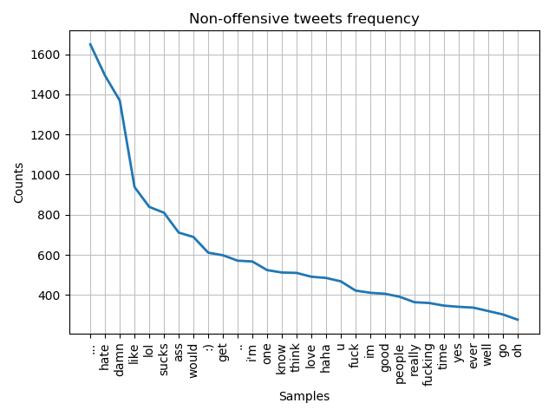
\includegraphics[width=3in]{non_offensive_tweets}
\caption{Most frequent words in non-offensive tweets.}
\label{non_off_dataset}
\end{figure}

\begin{figure}[!t]
\centering
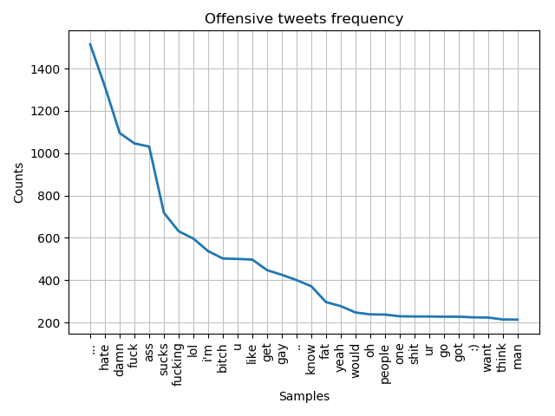
\includegraphics[width=3in]{offensive_tweets}
\caption{Most frequent words in offensive tweets.}
\label{off_dataset}
\end{figure}


\begin{figure}[!t]
\centering
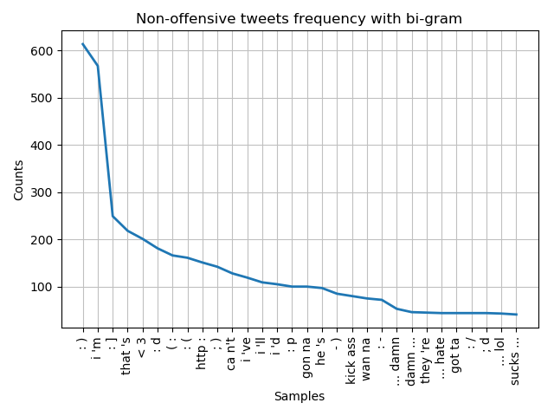
\includegraphics[width=3in]{non_offensive_tweets_bigram}
\caption{Most frequent words in non-offensive tweets grouped in bi-gram.}
\label{non_off_dataset_bigram}
\end{figure}

\begin{figure}[!t]
\centering
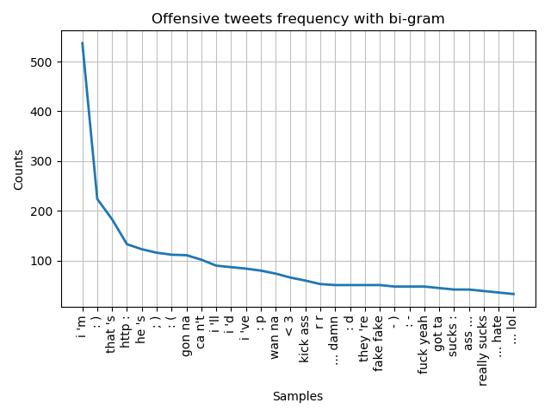
\includegraphics[width=3in]{offensive_tweets_bigram}
\caption{Most frequent words in offensive tweets grouped in bi-gram.}
\label{off_dataset_bigram}
\end{figure}

In the dataset there are 17576 unique tokens. In the non-offensive tweets there are 14922 unique tokens, while in the offensive tweets there are 6486 unique tokens. If we group tokens sequentially in groups of two (bi-gram), there are 77973 unique tokens. In the non-offensive tweets there are 62609 unique tokens and in the offensive tweets there are 18458 unique tokens.

\section{Data pre-processing}
The pre-processing of words is done using a series of transformations applied to the words in the tweets. This step is fundamental to the normalization of words with similar meaning and remotion of unnecessary words in the tweets. First, all characters in tweets are lowercased. To each tweet is applied a tokenizer to split the tweets in words and convert the words into tokens. In this case, it was applied the TweetTokenizer, present in the NLTK library \footnote{\url{https://www.nltk.org/api/nltk.tokenize.html}}.

Afterwards, the punctuation is removed from the tokens, as well as the stop words ("the", "and", "of", ...). The stop words used are from the Stopwords Corpus in NLTK library. Finally, a lemmatization algorithm is applied to the tokens, to group the inflected forms of a word for better analysis of different words with the same meaning. The algorithm used was WordNet Lemmatizer, also included in the NLTK library \footnote{\url{https://wordnet.princeton.edu/}}. Instead of lemmatization, stemming could also be used, but lemmatization was chosen because of the use of a vocabulary dictionary and morphological analysis to get a better representation of the words.

\section{Feature extraction}
To extract the features from the tokens in tweets two methods were used:
\begin{itemize}
\item N-gram counting;
\item TF-IDF weighting.
\end{itemize}

The first method involves couting and selecting the top most used tokens in the tweets and use them as features. The related feature will be the number of times the tweet contains each one of the tokens. The result will be a sparse matrix that is normalized after all the countings. To include token proximity, it is tested with 1-gram and 2-gram tokens and it will be evaluated if the general results of the model improve with 2-gram tokens. N-gram groups a contiguous sequence of N tokens. We have chosen to take a word as the basic unit. For example, the tweet with the tokens "we", "love" and "ai" can be transformed into "we love" and "love ai" 2-gram tokens. With that, the token locality can be better represented. This behavior was achieved with the use of CountVectorizer module in Scikit-learn library \footnote{\url{https://scikit-learn.org/stable/modules/generated/sklearn.feature_extraction.text.CountVectorizer.html}}.

The second method involves calculating the TF-IDF (term frequency – inverse document frequency) and selecting the top most used tokens in the tweets, using the weight of each token in a tweet as feature. The TF-IDF is as term-weighting scheme used to represent the importance of a token in a tweet. The importance of a term increases logarithmically with its frequency in a tweet and the weight is normalized according to all other weights in the same tweet, being unnecessary further normalization. This behaviour was achieved with the use of TfidfVectorizer module in Scikit-learn library \footnote{\url{https://scikit-learn.org/stable/modules/generated/sklearn.feature_extraction.text.TfidfVectorizer.html}}.

\section{Training \& Testing}

\subsection{Training approach}

The dataset division for the training and testing phase was 80\% of data for training and cross-validation (using five-fold cross-validation) and 20\% for testing.

Different classifiers and parameters were tested.

The tested classifiers were:
\begin{itemize}
\item Logistic Regression;
\item SGD Classifier;
\item Linear SVC;
\item NuSVC;
\item SVC;
\item Gaussian Naive Bayes;
\item Decision Tree;
\item Random Forest;
\item AdaBoost;
\item XGBoost;
\item Multi-layer Perceptrons.
\end{itemize}

The different parameters to test were:
\begin{itemize}
\item Maximum number of most used tokens to create features;
\item Different n-gram parameters for N-gram counting (1-gram, 2-gram and combination);
\item N-gram counting and TF-IDF weighting combination;
\item Classifiers hyperparameters.
\end{itemize}

Due to the many classifiers chosen to evaluate, the number of possible parameter combinations has an exponential growth, being virtually impossible to make an optimal evaluation.

To solve that problem, the evaluation phase was subdivided in a sub-optimal 3-step phase described below.

\subsection{First evaluation phase}

On the first phase, the classifiers are tested using the default hyperparameters. The use of the N-gram counting and TF-IDF weighting approaches are tested separately and combined. The number of most used tokens vary between 100, 1000, 5000, 10000 and 25000. This number is used to give a maximum number of tokens used in the feature extraction. The tests are also done using 1-gram tokens, 2-gram tokens and both approaches combined (only applied to the N-gram counting).
Finally, for each test, it is performed five-fold cross-validation using 80\% of the dataset and is stored the confusion matrix, accuracy, precision, recall and f1-score. The most important metrics for the problem are accuracy and recall. A high recall is essential because if the classifier has many false positives, they can be detected by manual inspection. However, if the classifier produces many false negatives, they will not be analyzed and they will perturb readers.

On this phase, the best combination of parameters is chosen, along with the four classifiers with the best results.

\subsection{Second evaluation phase}

On the second phase, the four best classifiers from the first phase are tested with different hyperparameters. This phase is for selecting the best hyperparameters for each one of the classifiers based on the obtained results, also using five-fold cross-validation.

\subsection{Third evaluation phase}

On the last phase, the four best classifiers with the best hyperparameters and features will be tested with 20\% of the dataset, the test data, to get the final results.

\subsection{First testing phase}

The extensive results of the first testing phase can be found in the Appendix \ref{AppA}.

In this phase, some classifiers were only tested with the number of most used tokens below 5000, being removed from this analysis. NuSVC and SVC were eliminated due to the excessive memory used (due to the kernel transformations), causing a memory error (NuSVC and SVC are SVM's with polynomial kernel and Linear SVC was kept because it uses an SVM with a linear kernel). AdaBoost and XGBoost are two ensemble boosting methods that, due to the high number of features used, could not be trained in a reasonable time with a number of tokens higher than 5000.

In the figure \ref{averageAccFeatures} we can see the impact of choosing a different number of most used tokens to analyze. Better results are achieved when the number of tokens chosen to represent the features is higher.

However, other conclusions can be drawn from this figure. For a small number of tokens, the approaches with TF-IDF are the ones with the higher accuracy. While the performance of models that take into account bi-gram tokens improves the accuracy of the classifiers, the performance of the models that only take into account one-gram tokens seems to decrease after the 5000 most used tokens. This can happen because while the bi-gram tokens have 81075 unique tokens in both classes (62609 unique tokens in non-offensive tweets and 18458 unique tokens in offensive tweets), one-gram tokens only have 21408 unique tokens in both classes (14922 unique tokens in non-offensive tweets and 6486 unique tokens in offensive tweets). According to the Zipf's Law\footnote{\url{https://en.wikipedia.org/wiki/Zipf's_law}}, 80\% of the words in a document appear only once. Which means that in this case, we are only interested in the most used 20\% tokens, which are 16215 tokens using bi-gram tokens, and 4281 tokens using one-gram tokens. Increasing the number of one-gram tokens after 4281 tokens may only add noise to the model, adding unnecessary tokens to characterize the classes, only overfitting on the training data. On the other hand, the accuracy of the models using bi-gram tokens as features seems to increase logarithmically with the number of tokens used.

It can also be seen that the models with TF-IDF features improve approximately 0.01 when compared with the same model without TF-IDF features.

The highest accuracy is achieved with only 2-gram features in the tokens counting and using TF-IDF.

\begin{figure}[!t]
\centering
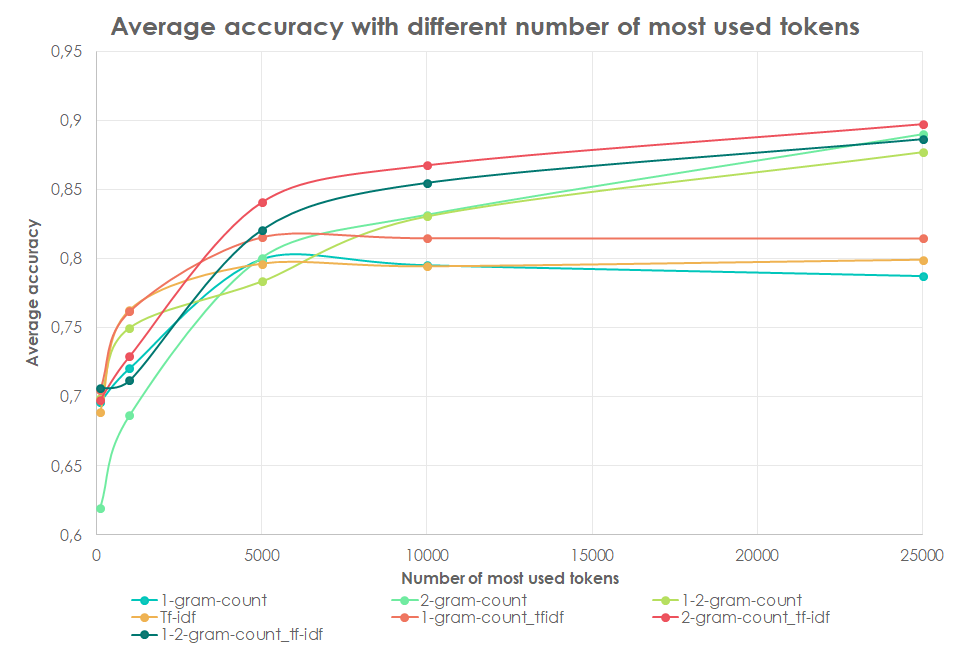
\includegraphics[width=3in]{AccFeatures_w}
\caption{Average accuracy with different number of features.}
\label{averageAccFeatures}
\end{figure}

The results for all classifiers tested with bi-gram tokens in the tokens counting and TF-IDF as feature extractors are shown in the figure \ref{AllClassifiers2GramIDF}. The classifier with higher precision and accuracy is the Logistic Regression, tied with the Linear SVC in the accuracy. The other two chosen classifiers were the ones that have the best recall, which is the Decision Tree and the Multi-layer Perceptrons.

\begin{figure}[!t]
\centering
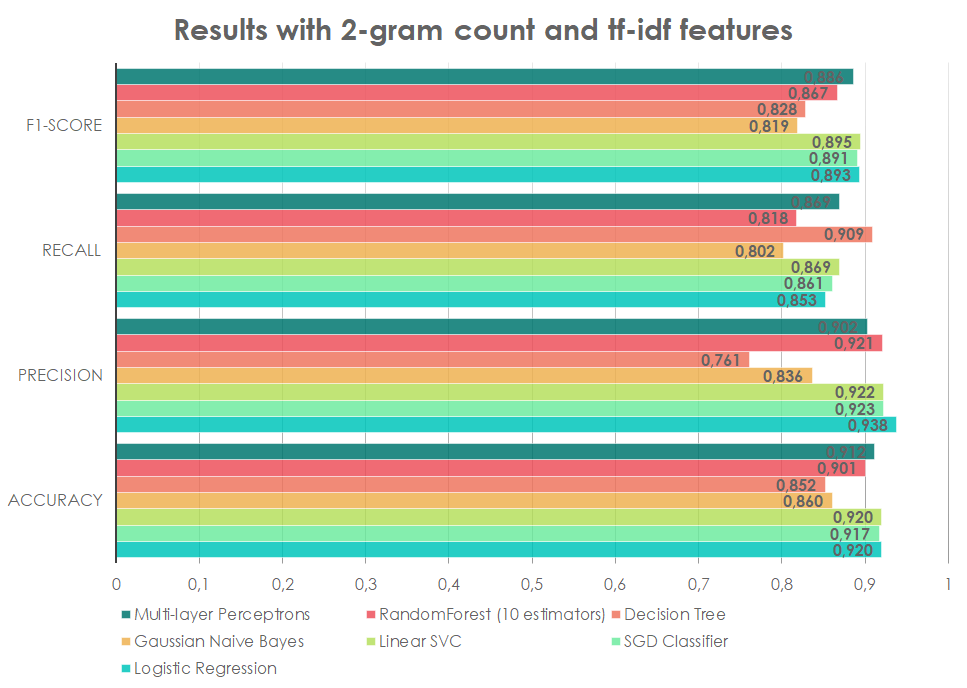
\includegraphics[width=3in]{AllClassifiers2GramIDF_w}
\caption{Full results of all classifiers with bi-gram tokens in the tokens counting and TF-IDF features.}
\label{AllClassifiers2GramIDF}
\end{figure}


\subsection{Second testing phase}

The four classifiers that are tested in this stage, as explained in the previous subsection, are Multi-layer Perceptrons, Decision Tree, Linear SVC and Logistic Regression.

The extensive results can be found the appendix \ref{AppB}.

\subsubsection{Multi-layer Perceptrons}
On the Multi-layer Perceptrons classifier, the following hyperparameters were chosen:
\begin{itemize}
\item Activation function: ReLU (Rectified Linear Unit);
\item Solver: ADAM;
\item 500 epochs for training, with early stopping.
\end{itemize}

The hyperparameters chosen to vary were:
\begin{itemize}
\item Network configuration;
\item Lambda value.
\end{itemize}

The network configuration varied among one, two and three layers, with different numbers of neurons: 100, 10x10, 20x20, 50x10, 10x10x10, 20x20x20 and 50x50x10. The lambda value chosen to regularize the activation function in each neuron varied among 0, 0.0001, 0.001, 0.01, 0.1 and 1.

The figure \ref{nnresultsvaryingnetwork} shows the results obtained when using different network configurations. The results are similar among the different configurations, but it can be perceived a small improvement in the precision with smaller networks, with the exception of the configuration with just one layer.

\begin{figure}[!t]
\centering
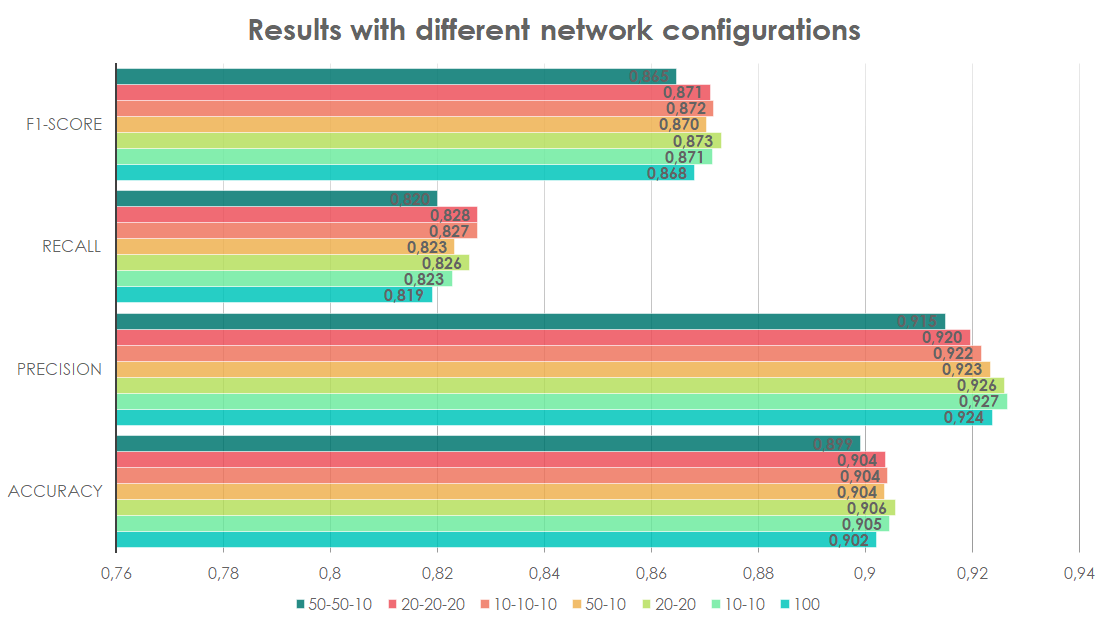
\includegraphics[width=3in]{nn1_w}
\caption{Multi-layer Perceptrons results using different network configurations.}
\label{nnresultsvaryingnetwork}
\end{figure}

In the figure \ref{nnresultsvaryinglambda} it can be seen the results of the classifier when tested with different lambda values. The results seem uncorrelated and the variations are too small to take any conclusion.

\begin{figure}[!t]
\centering
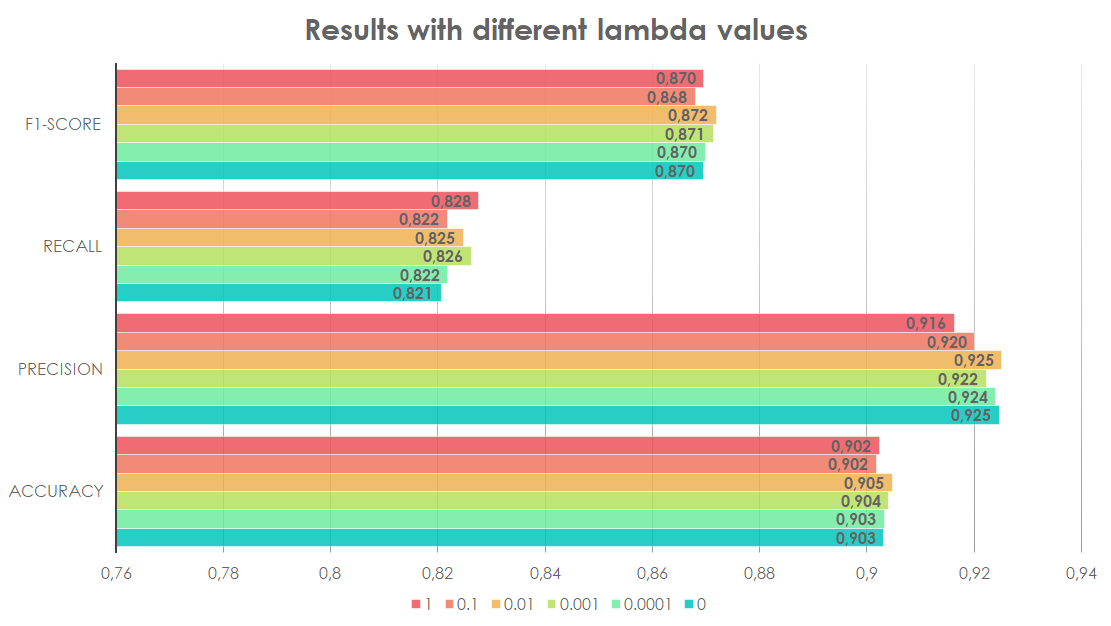
\includegraphics[width=3in]{nn2_w}
\caption{Multi-layer Perceptrons results using different lambda values.}
\label{nnresultsvaryinglambda}
\end{figure}

In the figure \ref{nnresultsfixednetworkvaryinglambda} the recall of the model is shown with different network configurations and lambda values. The recall is the chosen metric to represent because it is the most important metric to evaluate in this problem and in the previous tests showed worst results when compared with other metrics. Our goal is to maximize the recall, since the overall accuracy, F1-score and precision showed equally better results. It can be seen that the results with different network configurations and lambda values do not change dramatically among each other. However, the network with two layers and twenty neurons in each layer and a lambda value of 0.001 showed the highest recall. These parameters are the parameters chosen to calculate the final test result.

\begin{figure}[!t]
\centering
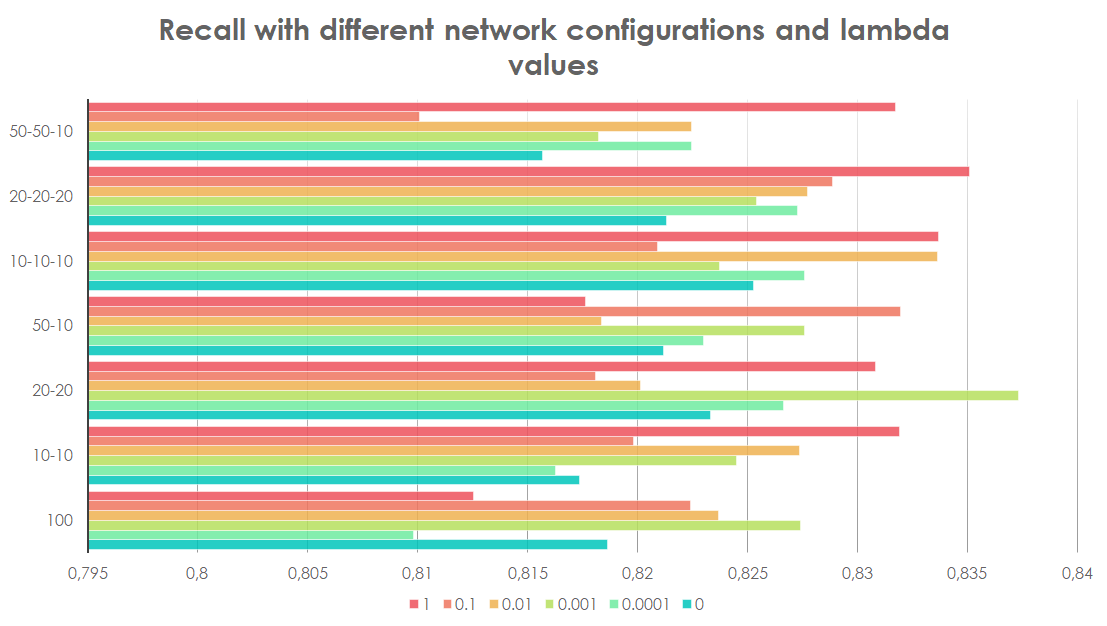
\includegraphics[width=3in]{nn3_w}
\caption{Multi-layer Perceptrons recall using different network configurations and lambda values.}
\label{nnresultsfixednetworkvaryinglambda}
\end{figure}

\subsubsection{Decision Tree}
On the Decision Tree classifier, the hyperparameters to vary were the following:
\begin{itemize}
\item Criterion;
\item Maximum depth.
\end{itemize}

The first hyperparameters specifies the function to measure the quality of a split. While "gini" uses the Gini impurity, "entropy" uses the information gain.
The second hyperparameter specifies the maximum depth of the tree. A few parameters were tested: 100, 200, 400, 600 and no maximum depth (more than 750 tree depth for both entropies tested, represented by 800).

The results when varying the maximum depth of the tree are presented in the figure \ref{dtvaryingdepth}. No conclusion can be taken from the results, because there is no clear trend in the data, the variations of results are minimal and seem totally random.

\begin{figure}[!t]
\centering
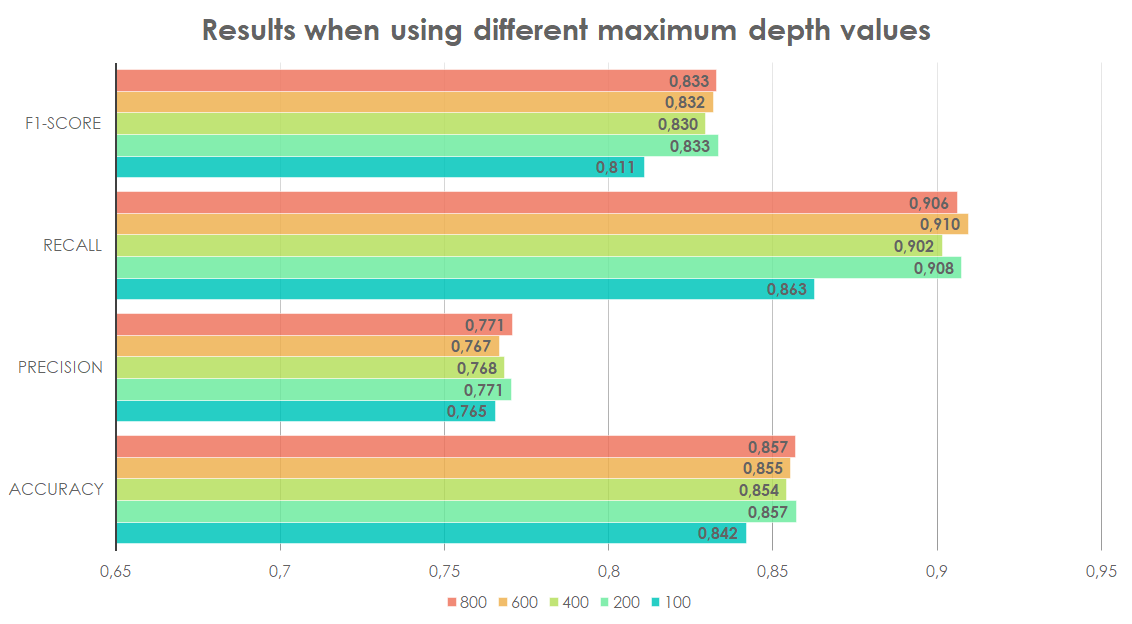
\includegraphics[width=3in]{dt1_w}
\caption{Decision Tree results using different maximum depth values.}
\label{dtvaryingdepth}
\end{figure}

In the figure \ref{dtvaryingcriterion} are compared the results when using entropy and gini criterion for splitting nodes. Entropy criterion presents better results for accuracy, precision, and F1-score. However, gini criterion has a higher recall. As recall is the most important metric to evaluate, the gini criterion will be chosen for the following tests on the classifier.

\begin{figure}[!t]
\centering
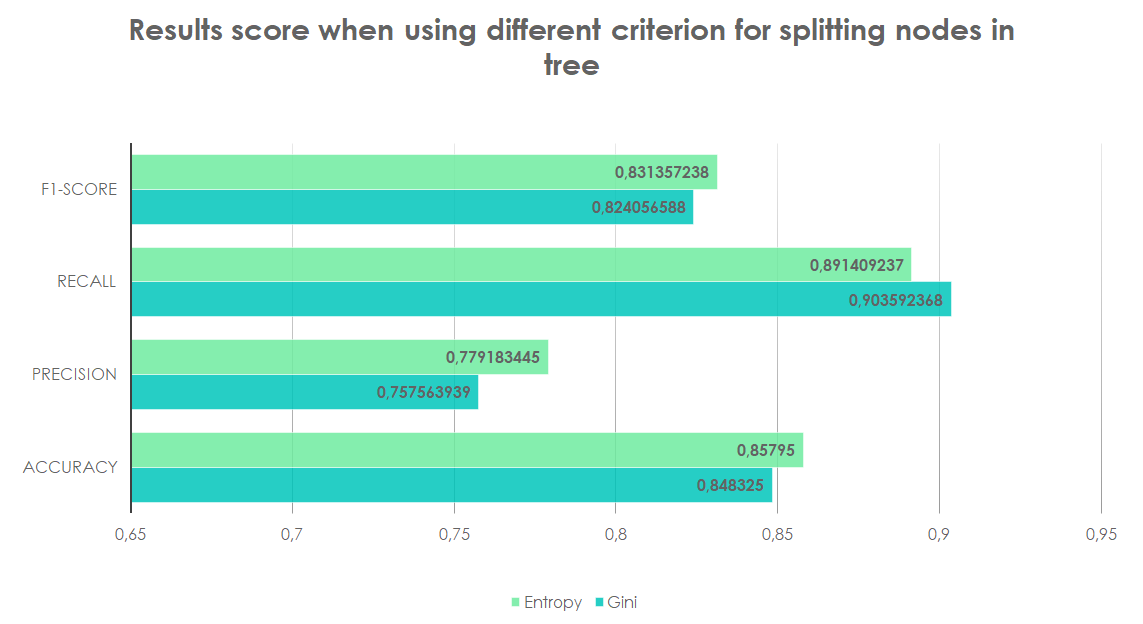
\includegraphics[width=3in]{dt2_w}
\caption{Decision Tree results using different criteria for splitting nodes.}
\label{dtvaryingcriterion}
\end{figure}

With gini as a criterion decision, the figure \ref{dtfixedcriterion} presents the results varying the maximum depth of the tree. It can be perceived a small improvement on the result with a higher tree depth. Particularly, the maximum depth chosen for the classifier is 600, because of the higher recall when compared with other tree depths.

\begin{figure}[!t]
\centering
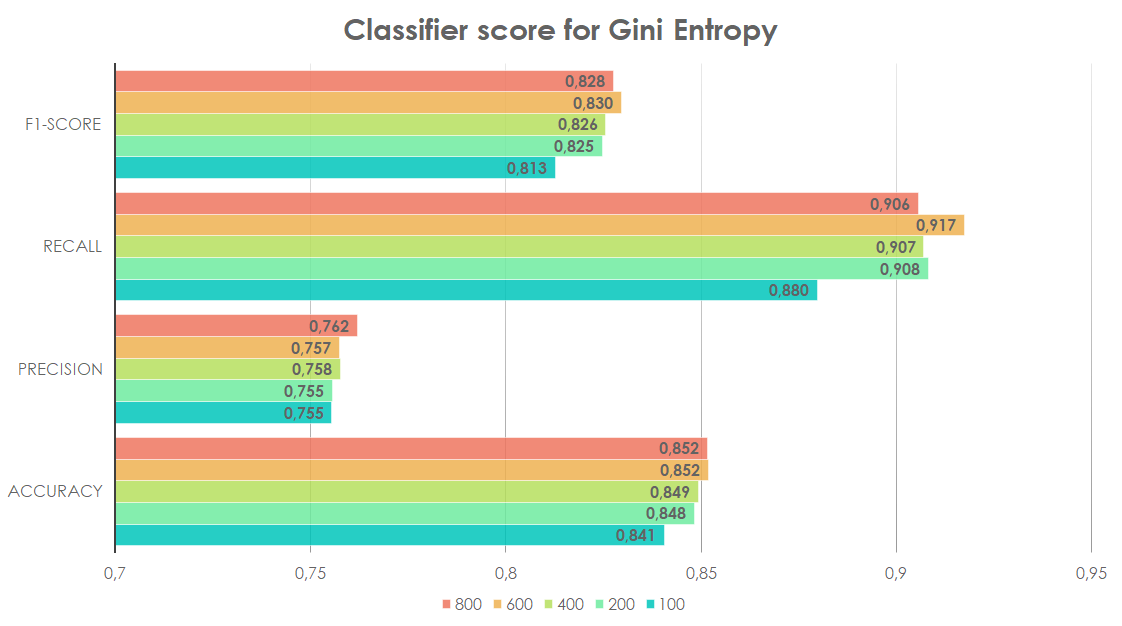
\includegraphics[width=3in]{dt3_w}
\caption{Decision tree results with gini criterion and varying the maximum tree depth.}
\label{dtfixedcriterion}
\end{figure}

\subsubsection{Linear SVC}
On the Linear SVC, the hyperparameters to vary were the following:
\begin{itemize}
\item Penalty;
\item C.
\end{itemize}

The first hyperparameter specifies the norm used in the penalization. It was tested with 'l1' and 'l2' penalties.
The second hyperparameter specifies the penalty parameter C of the error term. It determines the influence of the misclassification on the objective function. It was tested for the following values: 0.1, 1, 5, 10, 25, 50, 100, 500 and 1000.

In the figure \ref{lsvcaccuracy} it is shown the accuracy for l1 and l2 penalties with different C values. The highest accuracy value achieved for the l2 penalty was with C=5 and for the l1 penalty was with C=1. For the same penalty, the difference is insignificant between the values of C, except for C=0.1 using l1 penalty. We can conclude that the l2 penalty has better accuracy compared to the l1 penalty for almost all C values. For this reason, it is clear that the classifier will produce better results when applied l2 normalization.

\begin{figure}[!t]
\centering
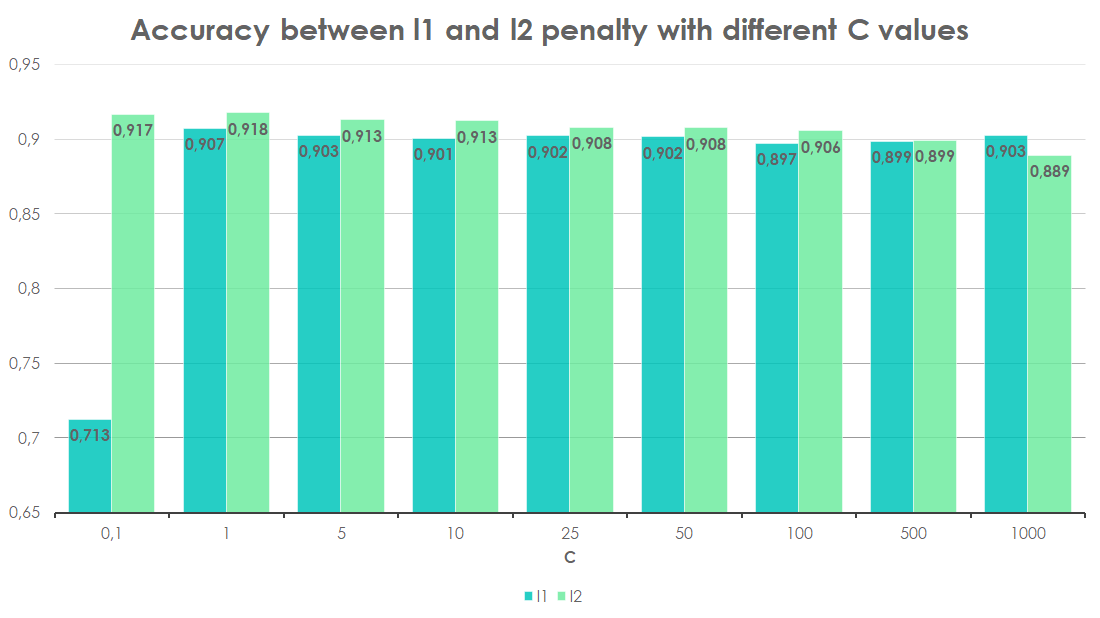
\includegraphics[width=3in]{lsvc1_w}
\caption{Linear SVC accuracy for l1 and l2 penalty with different C values.}
\label{lsvcaccuracy}
\end{figure}

In the figure \ref{lsvcaprf} it is shown the accuracy, precision, recall and f1-score values for different C values with l2 penalty. All parameters tend to decrease as C increases, with the exception of the recall. As accuracy and recall are the most important parameters in this problem, the most balanced combination must be evaluated. The highest accuracy value achieved was with C=0.1 but it has the worst recall. C=5 has the second highest accuracy result and a high recall. For this reason, we can conclude that C=5 offers the best relation between the two most important parameters referred above.

\begin{figure}[!t]
\centering
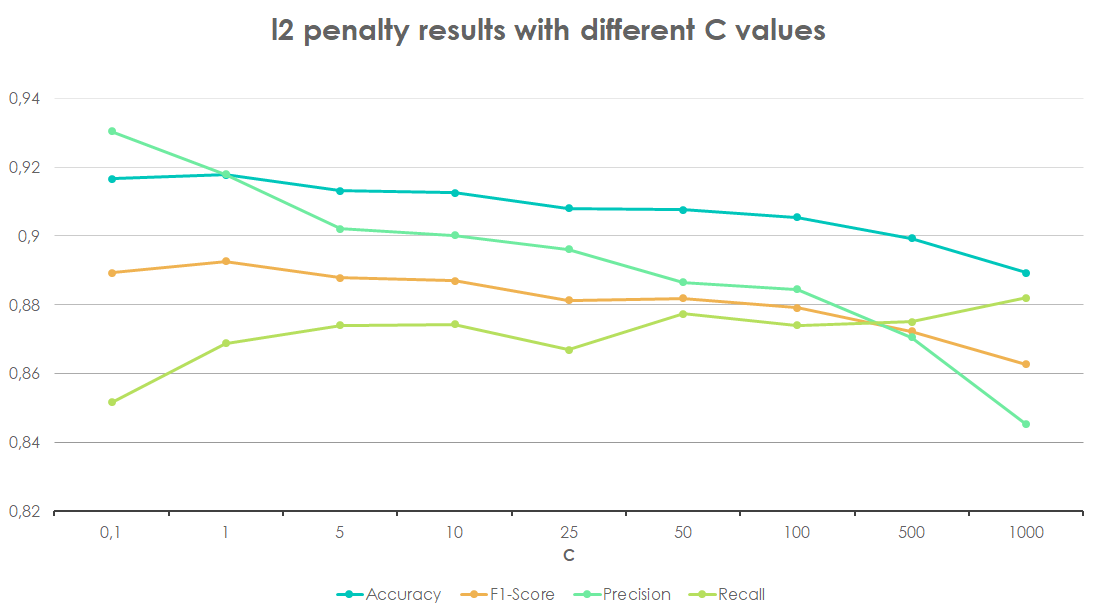
\includegraphics[width=3in]{lsvc2_w}
\caption{Linear SVC accuracy, precision, recall and f1-score for l2 penalty with different C values.}
\label{lsvcaprf}
\end{figure}

Based on the results shown, the best parameter values are l2 penalty and C=5.

\subsubsection{Logistic Regression}
On the Logistic Regression, the hyperparameters to vary were the following:
\begin{itemize}
\item Penalty;
\item C.
\end{itemize}

The first hyperparameter specifies the norm used in the penalization. It was tested with 'l1' and 'l2' penalties. The second hyperparameter specifies the penalty parameter C of the error term. It determines the influence of the misclassification on the objective function. It was tested for the following values: 0.1, 1, 5, 10, 25, 50, 100, 500 and 1000.

In the figure \ref{lraccuracy} it is shown the accuracy for l1 and l2 penalties with different C values. The highest accuracy value achieved for the l2 penalty was with C=5 and for the l1 penalty was with C=5 and C=10. We can conclude that the l2 penalty is the best choice because it has better accuracy compared to the l1 penalty for all C values.

\begin{figure}[!t]
\centering
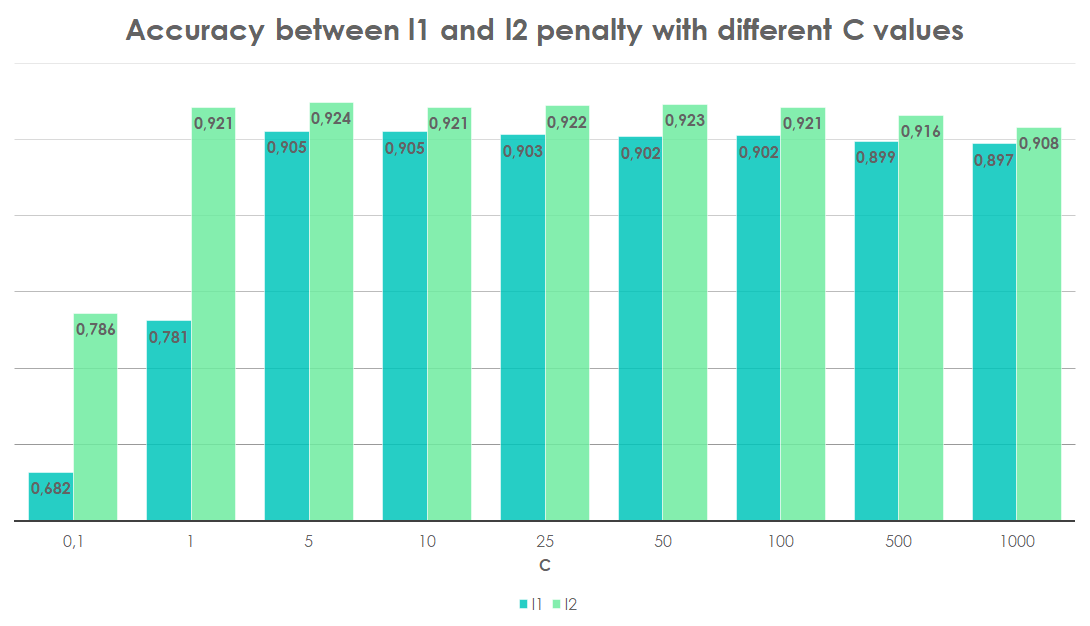
\includegraphics[width=3in]{lr1_w}
\caption{Logistic Regression accuracy for l1 and l2 penalty with different C values.}
\label{lraccuracy}
\end{figure}

In the figure \ref{lraprf} it is shown the accuracy, precision, recall and f1-score values for different C values. As referred before, accuracy and recall are the most important parameters in this problem, so it is preferred the most balanced combination. The highest accuracy value achieved was with C=1 but the difference is insignificant when compared to C=5. The highest recall value achieved was with C=50 or C=100. C=5 offers not only better accuracy that C=50 and C=100, but also better recall than C=1. It also has better accuracy than C=10 and C=25 and better recall that C=10, being almost the same as C=25. If we consider precision and f1-score, C=5 has the highest values overall. For this reasons, C=5 is considered the best C value, offering a balanced relation between accuracy and recall besides having the highest precision and f1-score.

\begin{figure}[!t]
\centering
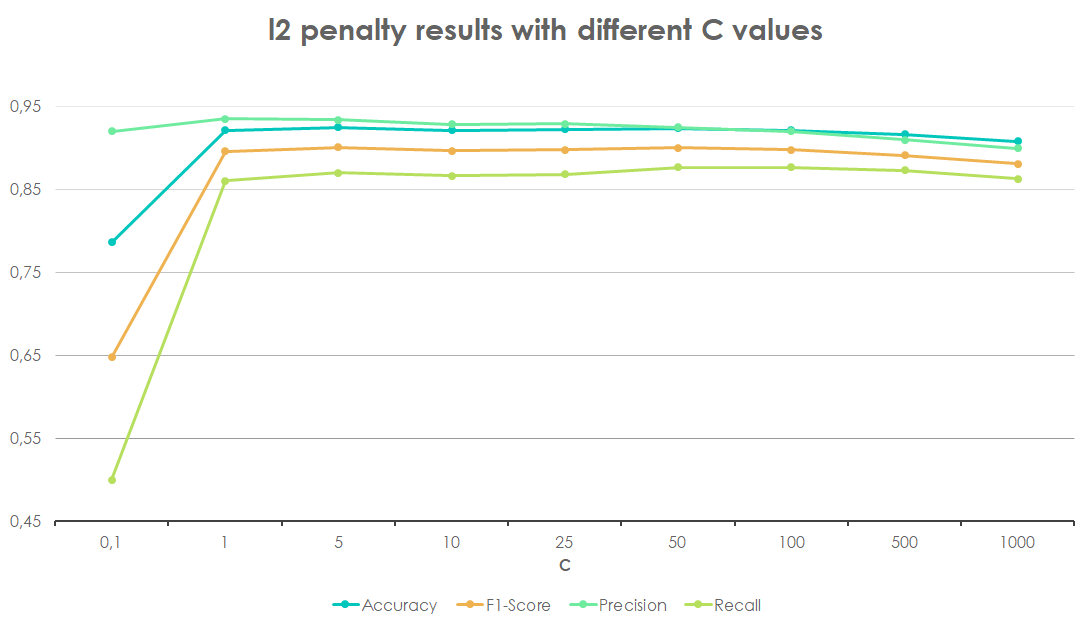
\includegraphics[width=3in]{lr2_w}
\caption{Logistic Regression accuracy, precision, recall and f1-score for l2 penalty with different C values.}
\label{lraprf}
\end{figure}

Based on the results shown, the best parameter values are l2 penalty and C=5.

\subsection{Final results}

In this subsection are presented the results of the final tests. These tests were made with 20\% of test data not used in the training phase, using the other 80\% data for training.

All results have improved in the final tests, due to the large amounts of data used for training. If a larger dataset was available, it would be interesting to train the classifiers with more data to test if the results improved even more.

In the table \ref{table:finalresults} it is possible to see the final results. The Logistic Regression presents the highest accuracy and f1-score, followed close by Linear SVC. The Decision Tree has the worst accuracy, precision and f1-score, but it presents the best recall. However, the Logistic Regression and LinearSVC recall are not far from the Decision Tree recall. The Multi-layer perceptrons have the higher precision value, but the worst recall.

From the analysis of the results, the Multi-layer Perceptrons would not be considered to the final classifier due to the low recall. The Logistic Regression and Linear SVC are two classifiers that could be used to classify offensive tweets. While its recall is not the best when compared to the Decision Tree recall, its results are close to the best and have a much higher accuracy than both other classifiers. Overall, if the recall was crucial when dealing with classification of offensive tweets, even if that meant a lot of false positives, Decision Tree was the chosen classifier. Otherwise, if overall accuracy and f1-score results were more important than recall, Logistic Regression or Linear SVC would be the best classifiers to solve the problem.

\begin{table}
\caption{Final results of the four best classifiers}
\begin{center}
 \begin{tabular}{||c c c c c||} 
 \hline
 Classifier & Accuracy & Precision & Recall & F1-Score \\ [0.5ex] 
 \hline\hline
 Logistic & 0.956 & 0.940 & 0.946 & 0.943 \\ 
 Regression & & & & \\
 \hline
 Linear SVC & 0.952 & 0.924 & 0.952 & 0.938 \\
 \hline
 Decision Tree & 0.871 & 0.764 & 0.959 & 0.850 \\
 \hline
 Multi-layer & 0.944 & 0.943 & 0.907 & 0.925 \\
 Perceptrons & & & & \\
 \hline
\end{tabular}
\end{center}
\label{table:finalresults}
\end{table}

\section{Conclusion}
In this report, it was shown an approach to build an offensive tweet classifier. The final results show that it is possible to build a classifier with high accuracy (95.6\%) or high recall (95.9\%) using a small dataset (20001 tweets) by applying classical machine learning techniques and feature and model tuning.
In the explored dataset, the token count with one-gram tokens decreases the overall accuracy if having more than 5000 tokens as features to the counter. However, using two-gram tokens improves the overall classifiers results logarithmically with an increase in the number of tokens. This result may indicate that in this specific dataset, the most used tokens used in both classes of tweets are similar, but if we use token proximity we can better differentiate both classes.
In the four classifiers chosen to vary the hyperparameters, the impact of the hyperparameters variations was reduced. This may happen due to the high number of tokens used to extract features (25000 tokens) and consequently the high number of features used in the classifiers (almost 40000 features).
The results can be further improved using other techniques. Using bigger n-grams and possibly joining with bi-gram tokens can help to higher the general accuracy. More labelled data can also help to differentiate between both classes. Using recurrent deep learning networks may also detect long-range dependencies not explored in this work.



% if have a single appendix:
%\appendix[Proof of the Zonklar Equations]
% or
%\appendix  % for no appendix heading
% do not use \section anymore after \appendix, only \section*
% is possibly needed

% use appendices with more than one appendix
% then use \section to start each appendix
% you must declare a \section before using any
% \subsection or using \label (\appendices by itself
% starts a section numbered zero.)
%



%\section{Proof of the First Zonklar Equation}
%Appendix one text goes here.

% you can choose not to have a title for an appendix
% if you want by leaving the argument blank
%\section{}
%Appendix two text goes here.


% use section* for acknowledgment
%\section*{Acknowledgment}


%The authors would like to thank...


% Can use something like this to put references on a page
% by themselves when using endfloat and the captionsoff option.
\ifCLASSOPTIONcaptionsoff
  \newpage
\fi



% trigger a \newpage just before the given reference
% number - used to balance the columns on the last page
% adjust value as needed - may need to be readjusted if
% the document is modified later
%\IEEEtriggeratref{8}
% The "triggered" command can be changed if desired:
%\IEEEtriggercmd{\enlargethispage{-5in}}

% references section

% can use a bibliography generated by BibTeX as a .bbl file
% BibTeX documentation can be easily obtained at:
% http://mirror.ctan.org/biblio/bibtex/contrib/doc/
% The IEEEtran BibTeX style support page is at:
% http://www.michaelshell.org/tex/ieeetran/bibtex
%\bibliographystyle{plainnat}
\bibliographystyle{IEEEtran}
% argument is your BibTeX string definitions and bibliography database(s)
\bibliography{references.bib}
%
% <OR> manually copy in the resultant .bbl file
% set second argument of \begin to the number of references
% (used to reserve space for the reference number labels box)
%\begin{thebibliography}

% \bibitem{IEEEhowto:kopka}
% H.~Kopka and P.~W. Daly, \emph{A Guide to \LaTeX}, 3rd~ed.\hskip 1em plus
%   0.5em minus 0.4em\relax Harlow, England: Addison-Wesley, 1999.

%\end{thebibliography}

% biography section
% 
% If you have an EPS/PDF photo (graphicx package needed) extra braces are
% needed around the contents of the optional argument to biography to prevent
% the LaTeX parser from getting confused when it sees the complicated
% \includegraphics command within an optional argument. (You could create
% your own custom macro containing the \includegraphics command to make things
% simpler here.)
%\begin{IEEEbiography}[{\includegraphics[width=1in,height=1.25in,clip,keepaspectratio]{mshell}}]{Michael Shell}
% or if you just want to reserve a space for a photo:

% \begin{IEEEbiography}{Michael Shell}
% Biography text here.
% \end{IEEEbiography}

% if you will not have a photo at all:
% \begin{IEEEbiographynophoto}{John Doe}
% Biography text here.
% \end{IEEEbiographynophoto}

% insert where needed to balance the two columns on the last page with
% biographies
%\newpage

%\begin{IEEEbiographynophoto}{Jane Doe}

%\end{IEEEbiographynophoto}

% You can push biographies down or up by placing
% a \vfill before or after them. The appropriate
% use of \vfill depends on what kind of text is
% on the last page and whether or not the columns
% are being equalized.

%\vfill

% Can be used to pull up biographies so that the bottom of the last one
% is flush with the other column.
%\enlargethispage{-5in}


\newpage
\appendices
\section{First testing phase results}
\label{AppA}
This appendix section contains seven pages, each one with different being tested.
\begin{itemize}
\item The first page contains the results only with 1-gram counter
\item The second page contains the results with 2-gram counter
\item The third page contains the results with 1-gram and 2-gram counter
\item The fourth page contains the results with TF-IDF
\item The fifth page contains the results with 1-gram counter and TF-IDF
\item The sixth page contains the results with 2-gram counter and TF-IDF
\item The seventh page contain the results with 1-gram and 2-gram counter and TF-IDF
\end{itemize}

Each table contains:
\begin{itemize}
\item Number of iteration
\item Number of features tested
\item Time to train (s)
\item True Positives (TP)
\item True Negatives (TN)
\item False Positives (FP)
\item False Negatives (FN)
\item Accuracy
\item Precision
\item Recall
\item F1-Score
\end{itemize}

\newpage
\clearpage

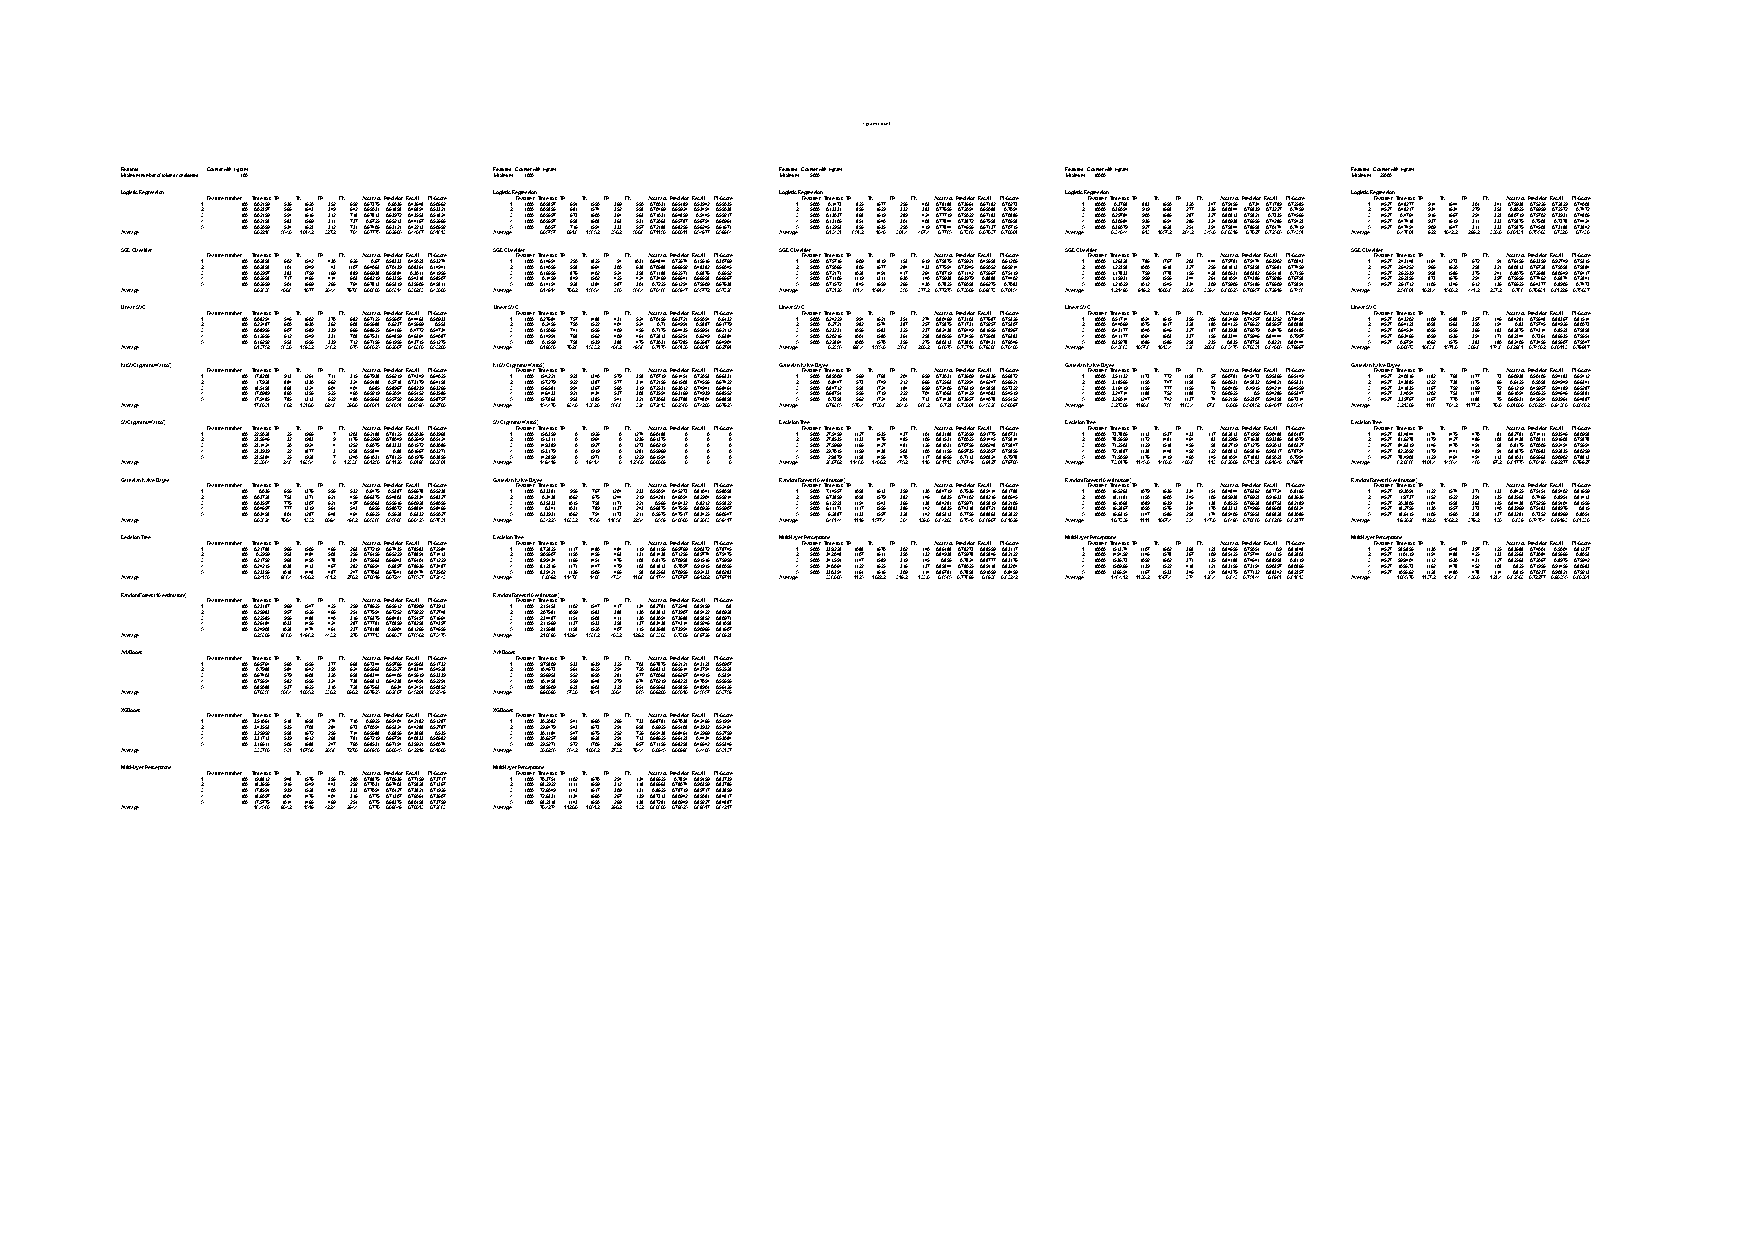
\includepdf[pages={-}, angle=90]{./First_Phase_Testing/Counter_1_gram.pdf}

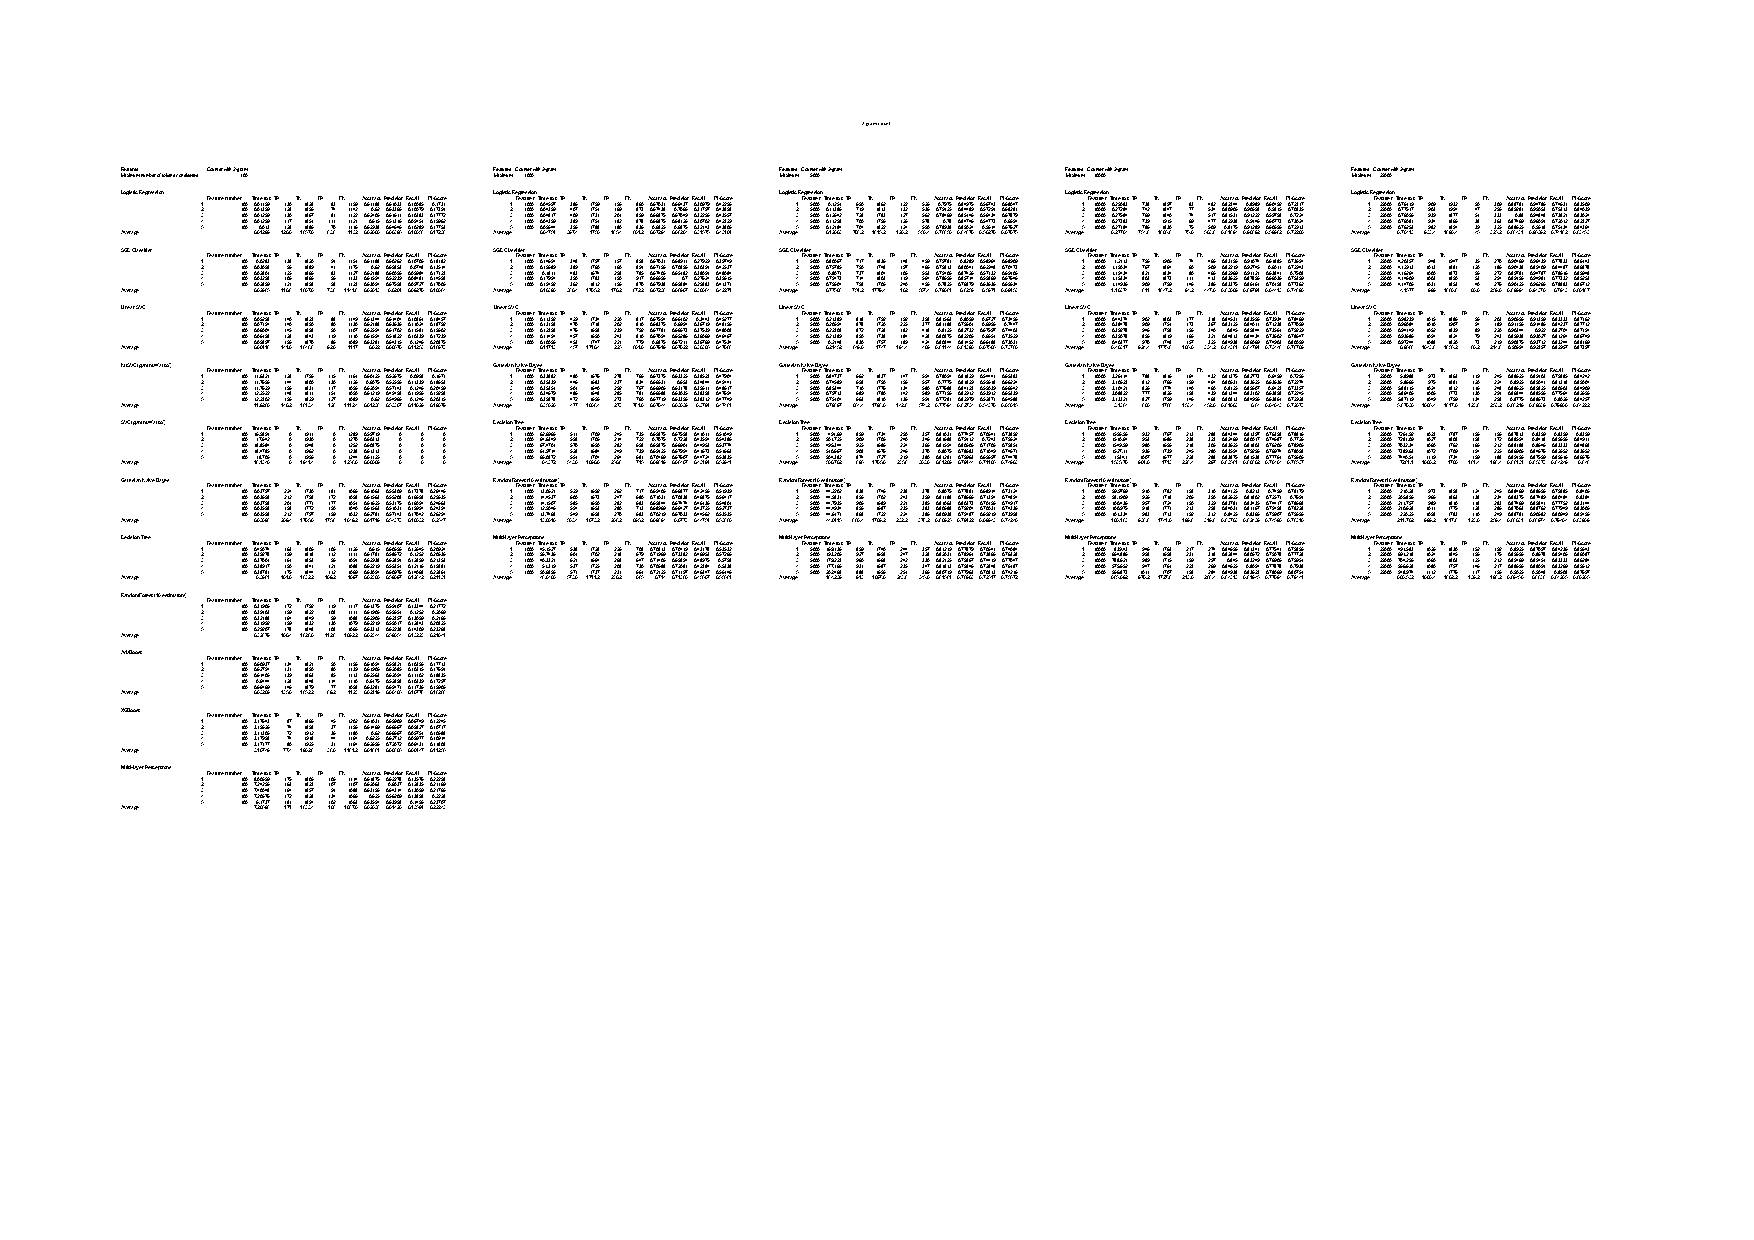
\includepdf[pages={-}, angle=90]{./First_Phase_Testing/Counter_2_gram.pdf}

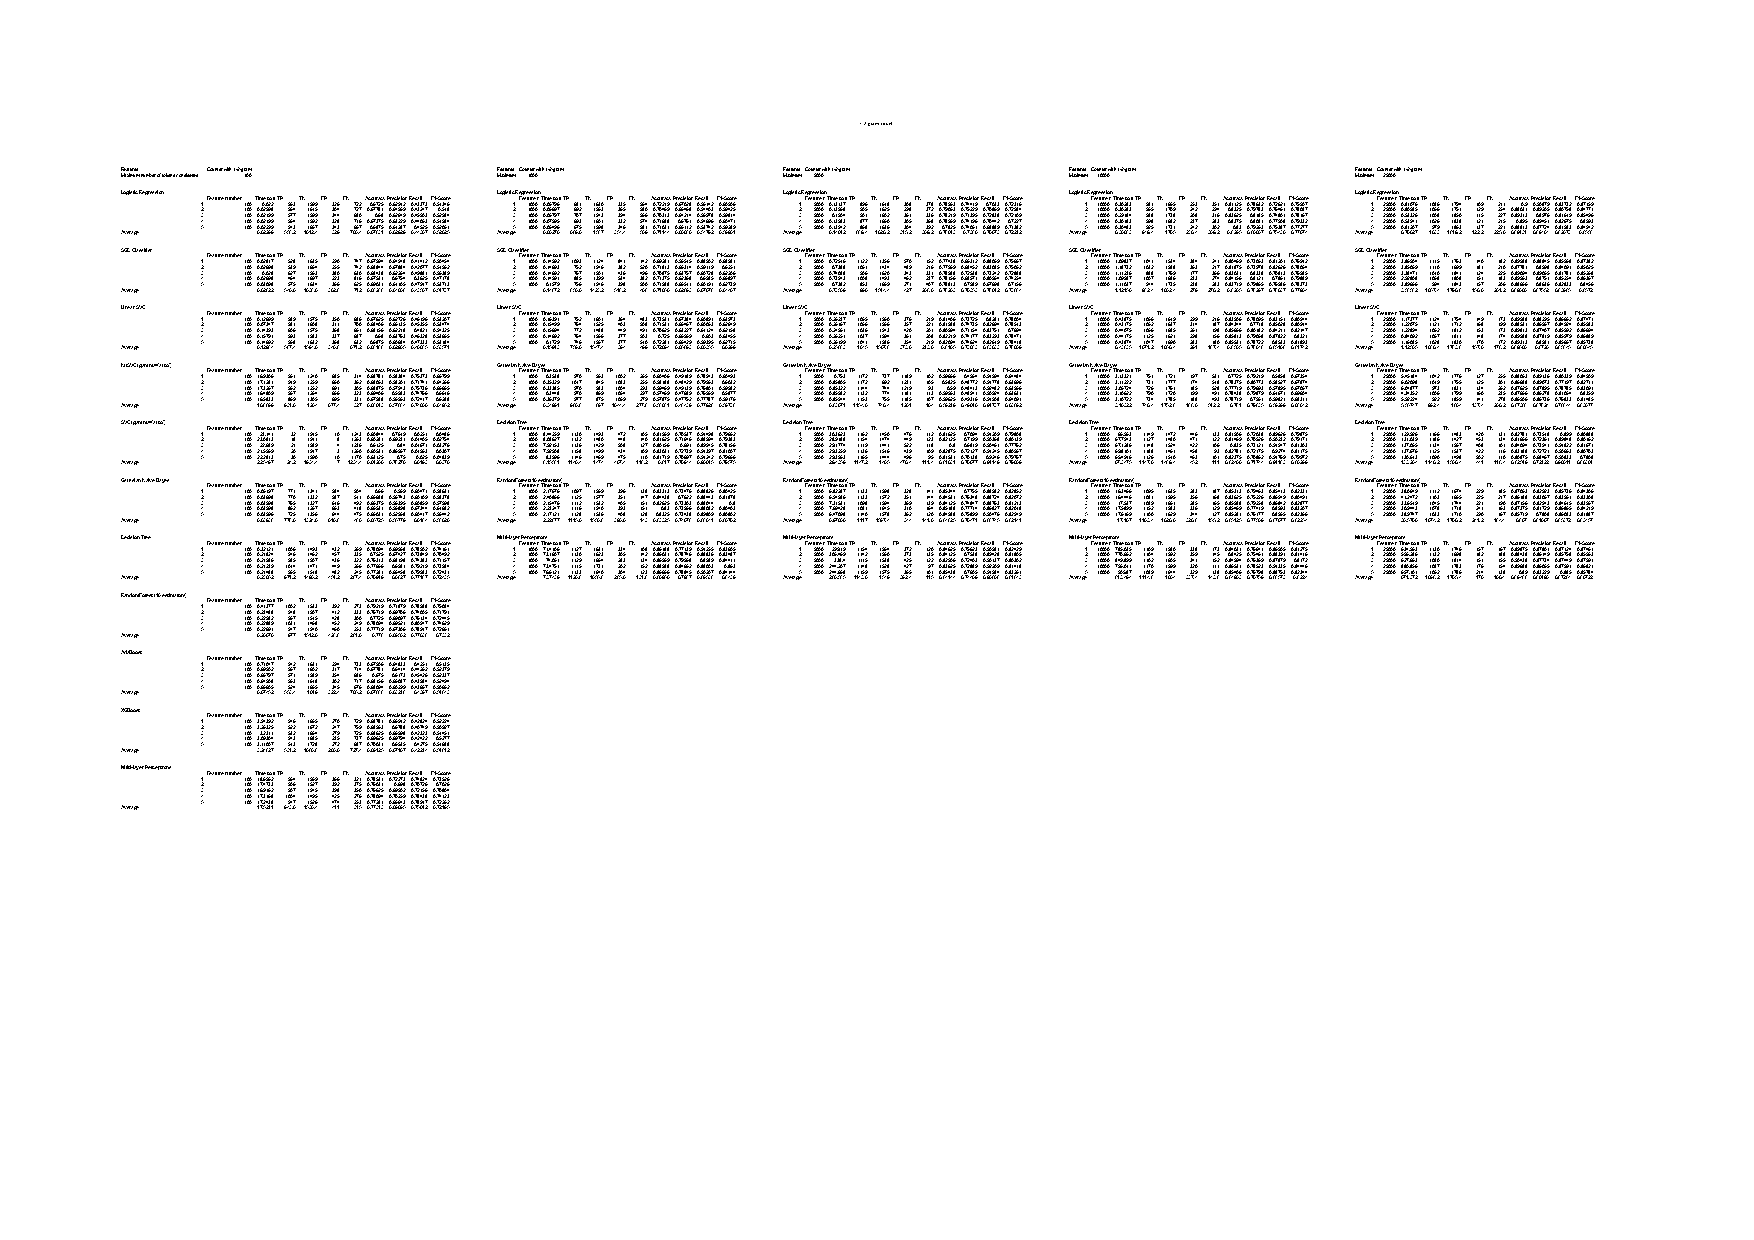
\includepdf[pages={-}, angle=90]{./First_Phase_Testing/Counter_1-2_gram.pdf}

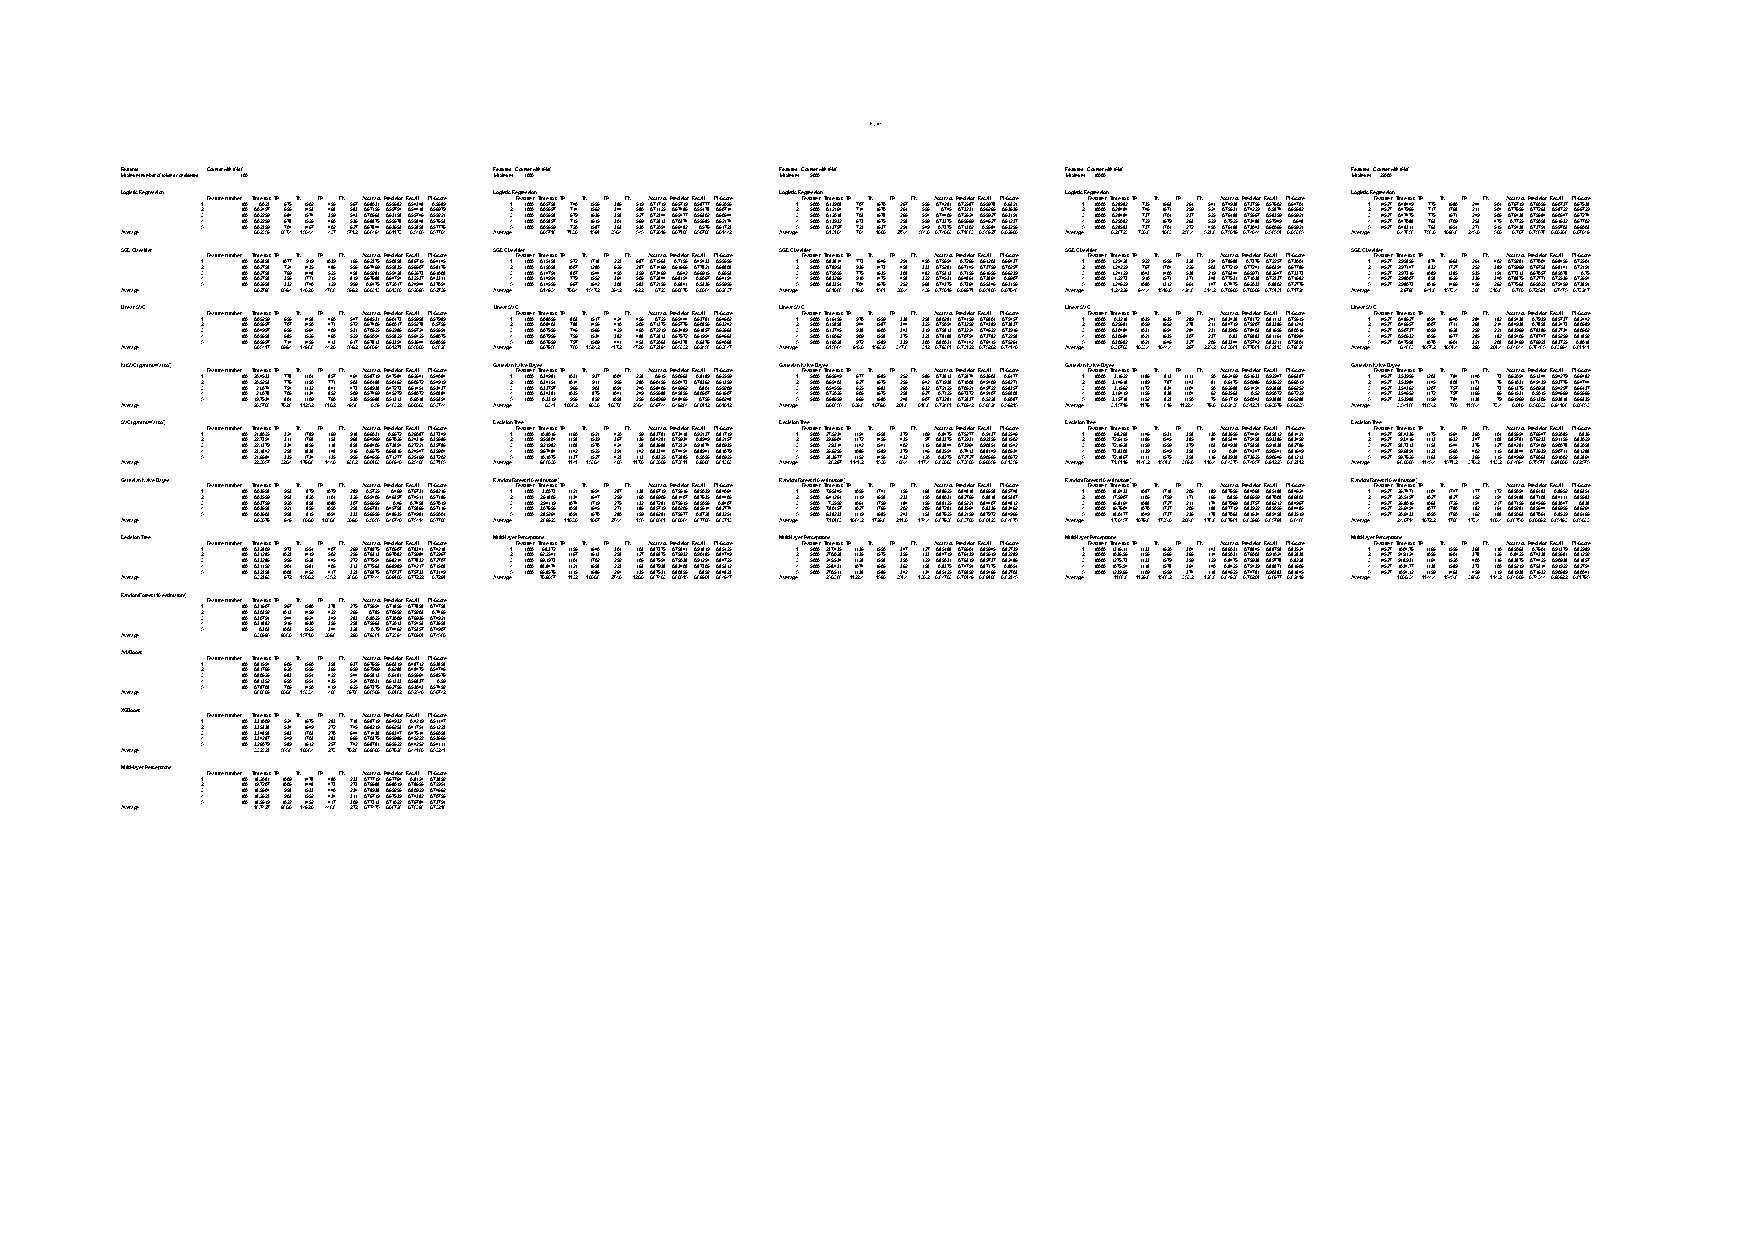
\includepdf[pages={-}, angle=90]{./First_Phase_Testing/TF-IDF.pdf}

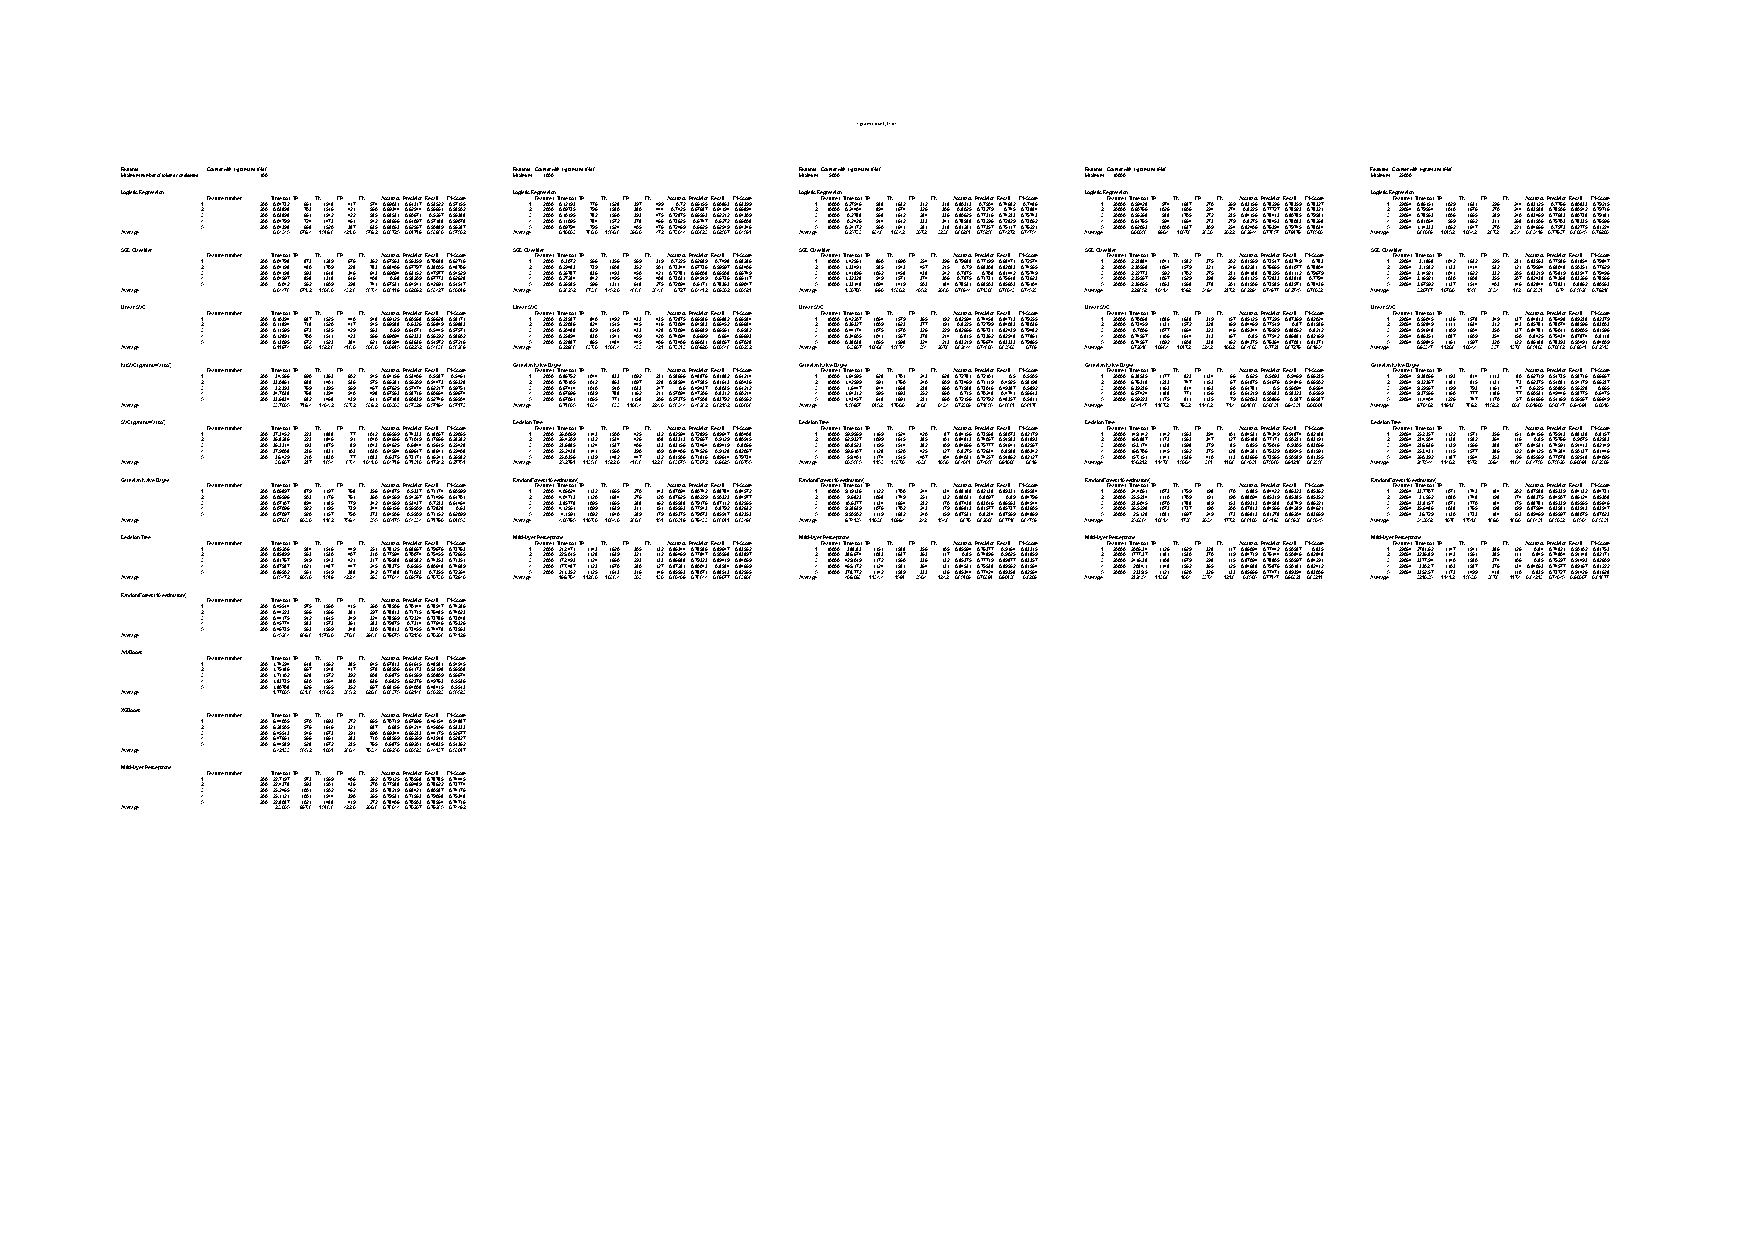
\includepdf[pages={-}, angle=90]{./First_Phase_Testing/Counter_1-gram_TF-IDF.pdf}

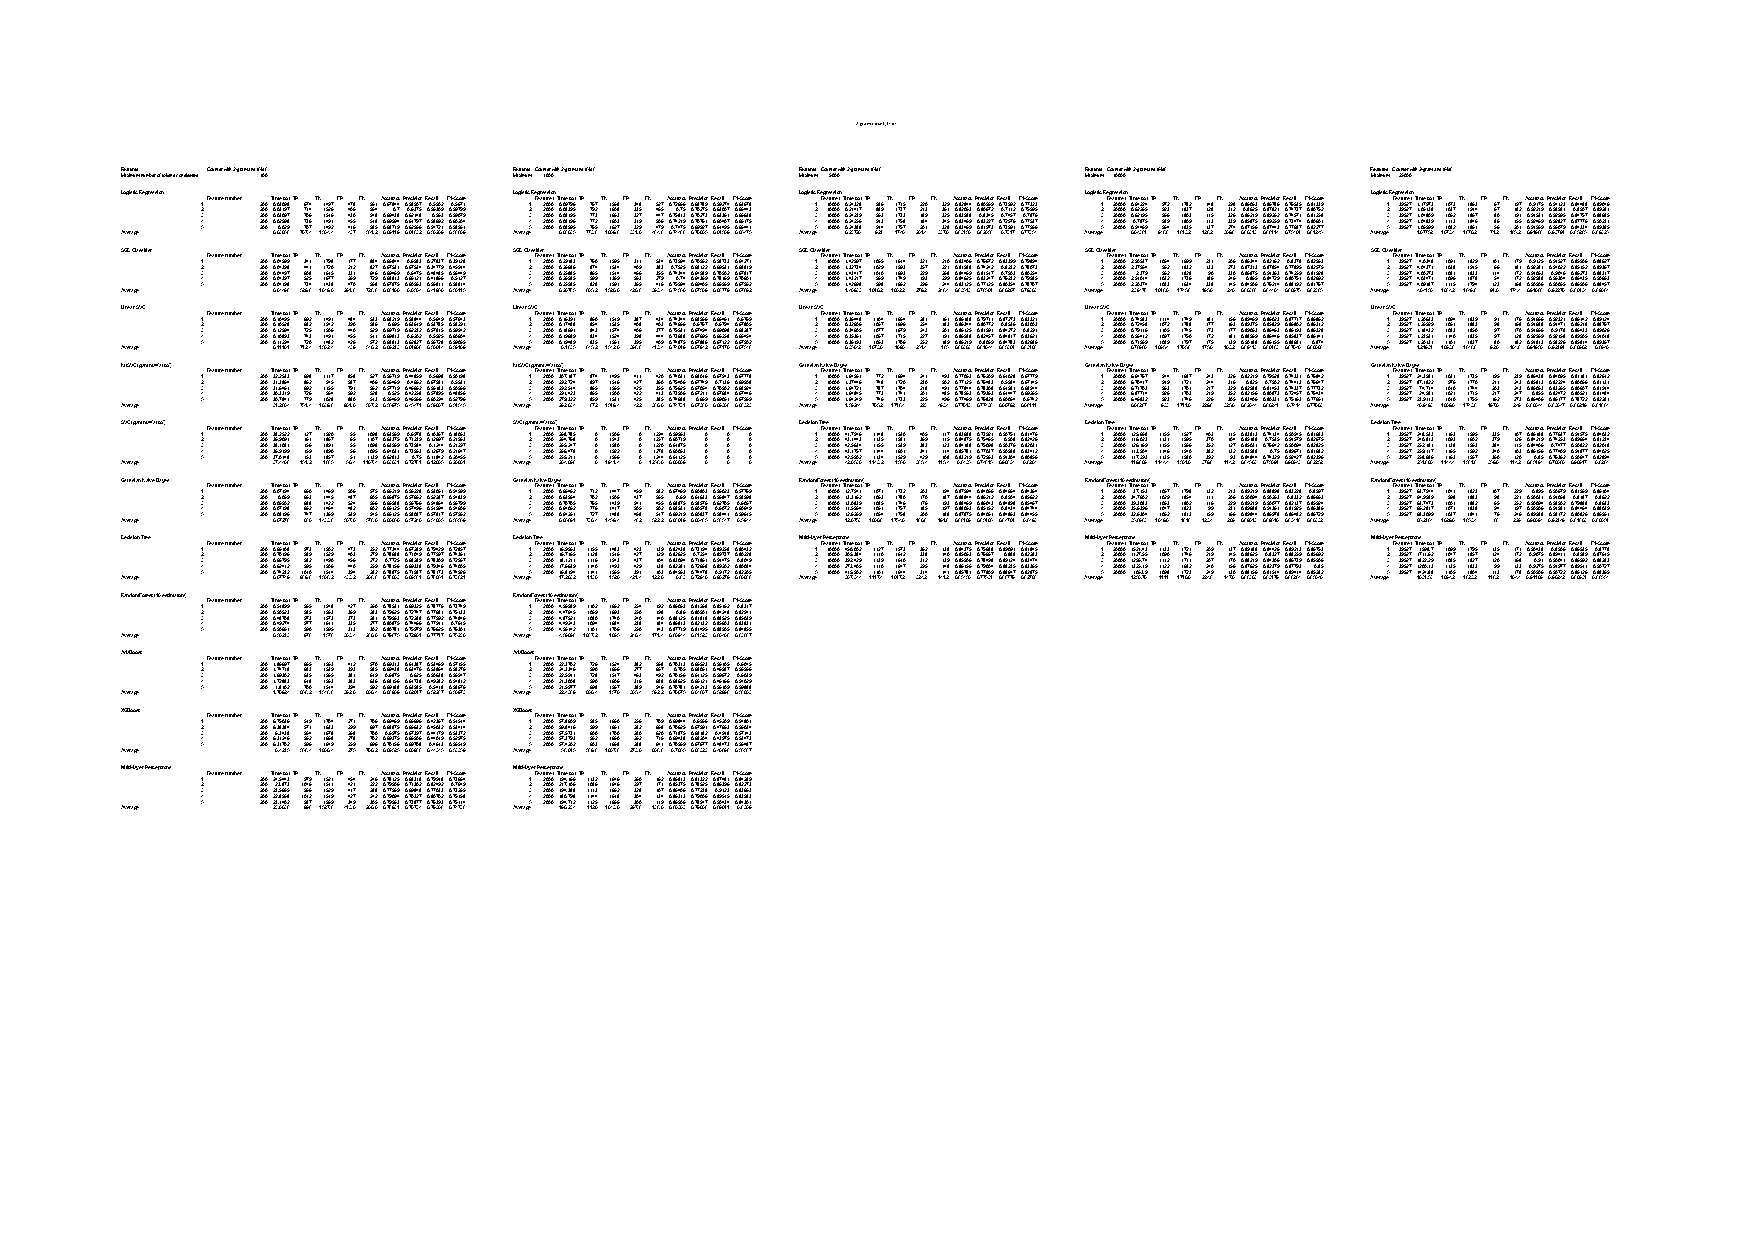
\includepdf[pages={-}, angle=90]{./First_Phase_Testing/Counter_2-gram_TF-IDF.pdf}

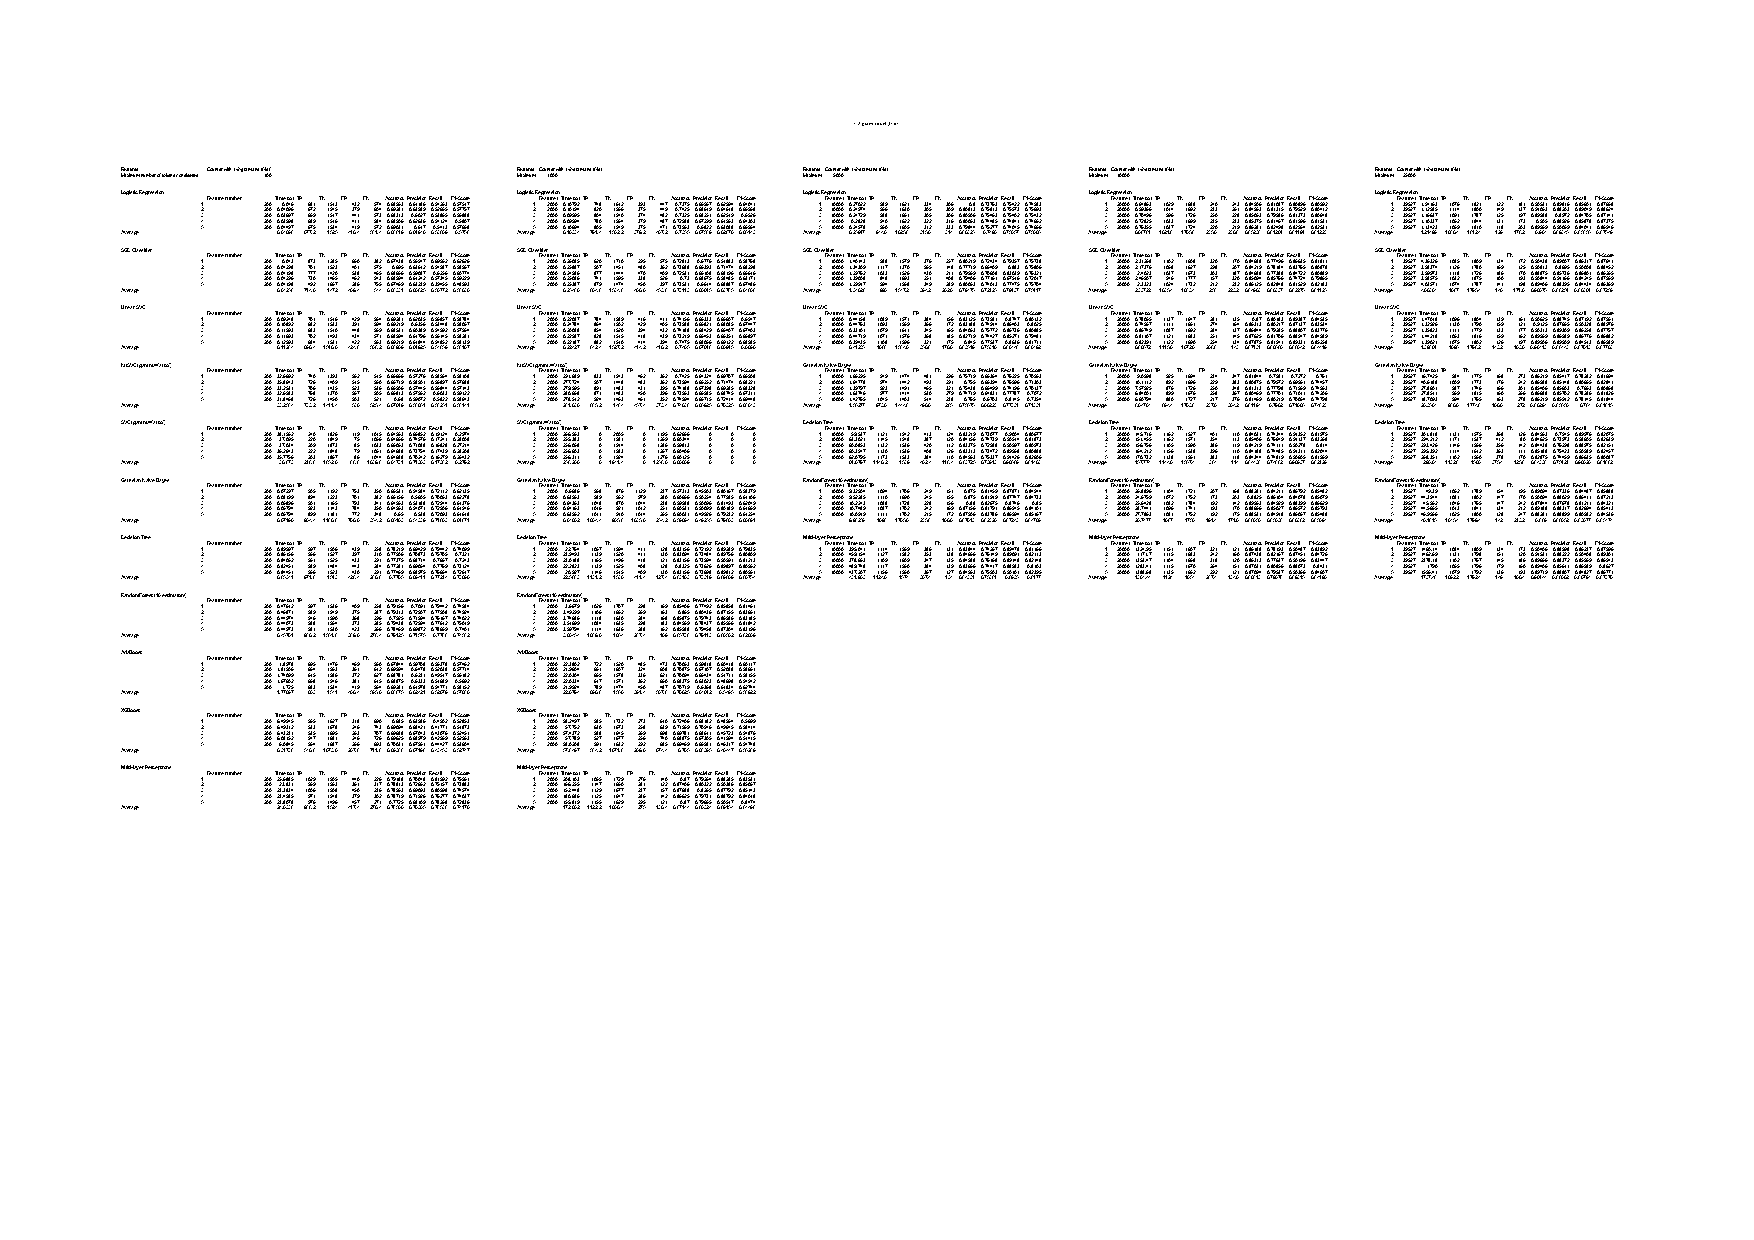
\includepdf[pages={-}, angle=90]{./First_Phase_Testing/Counter_1-2-gram_TF-IDF.pdf}

\section{Second testing phase results}
\label{AppB}
This appendix contains four pages, each one with the testing results with the changing of the hyperparameters of a classifier: Logistic Regression, Linear SVC, Decision Tree and Multi-layer Perceptrons, respectively.

Each table contains:
\begin{itemize}
\item Number of iteration
\item Number of features tested
\item Time to train (s)
\item True Positives (TP)
\item True Negatives (TN)
\item False Positives (FP)
\item False Negatives (FN)
\item Accuracy
\item Precision
\item Recall
\item F1-Score
\end{itemize}

\clearpage


\includepdf[pages={-}, angle=90]{./Second_Phase_Testing/LR.pdf}
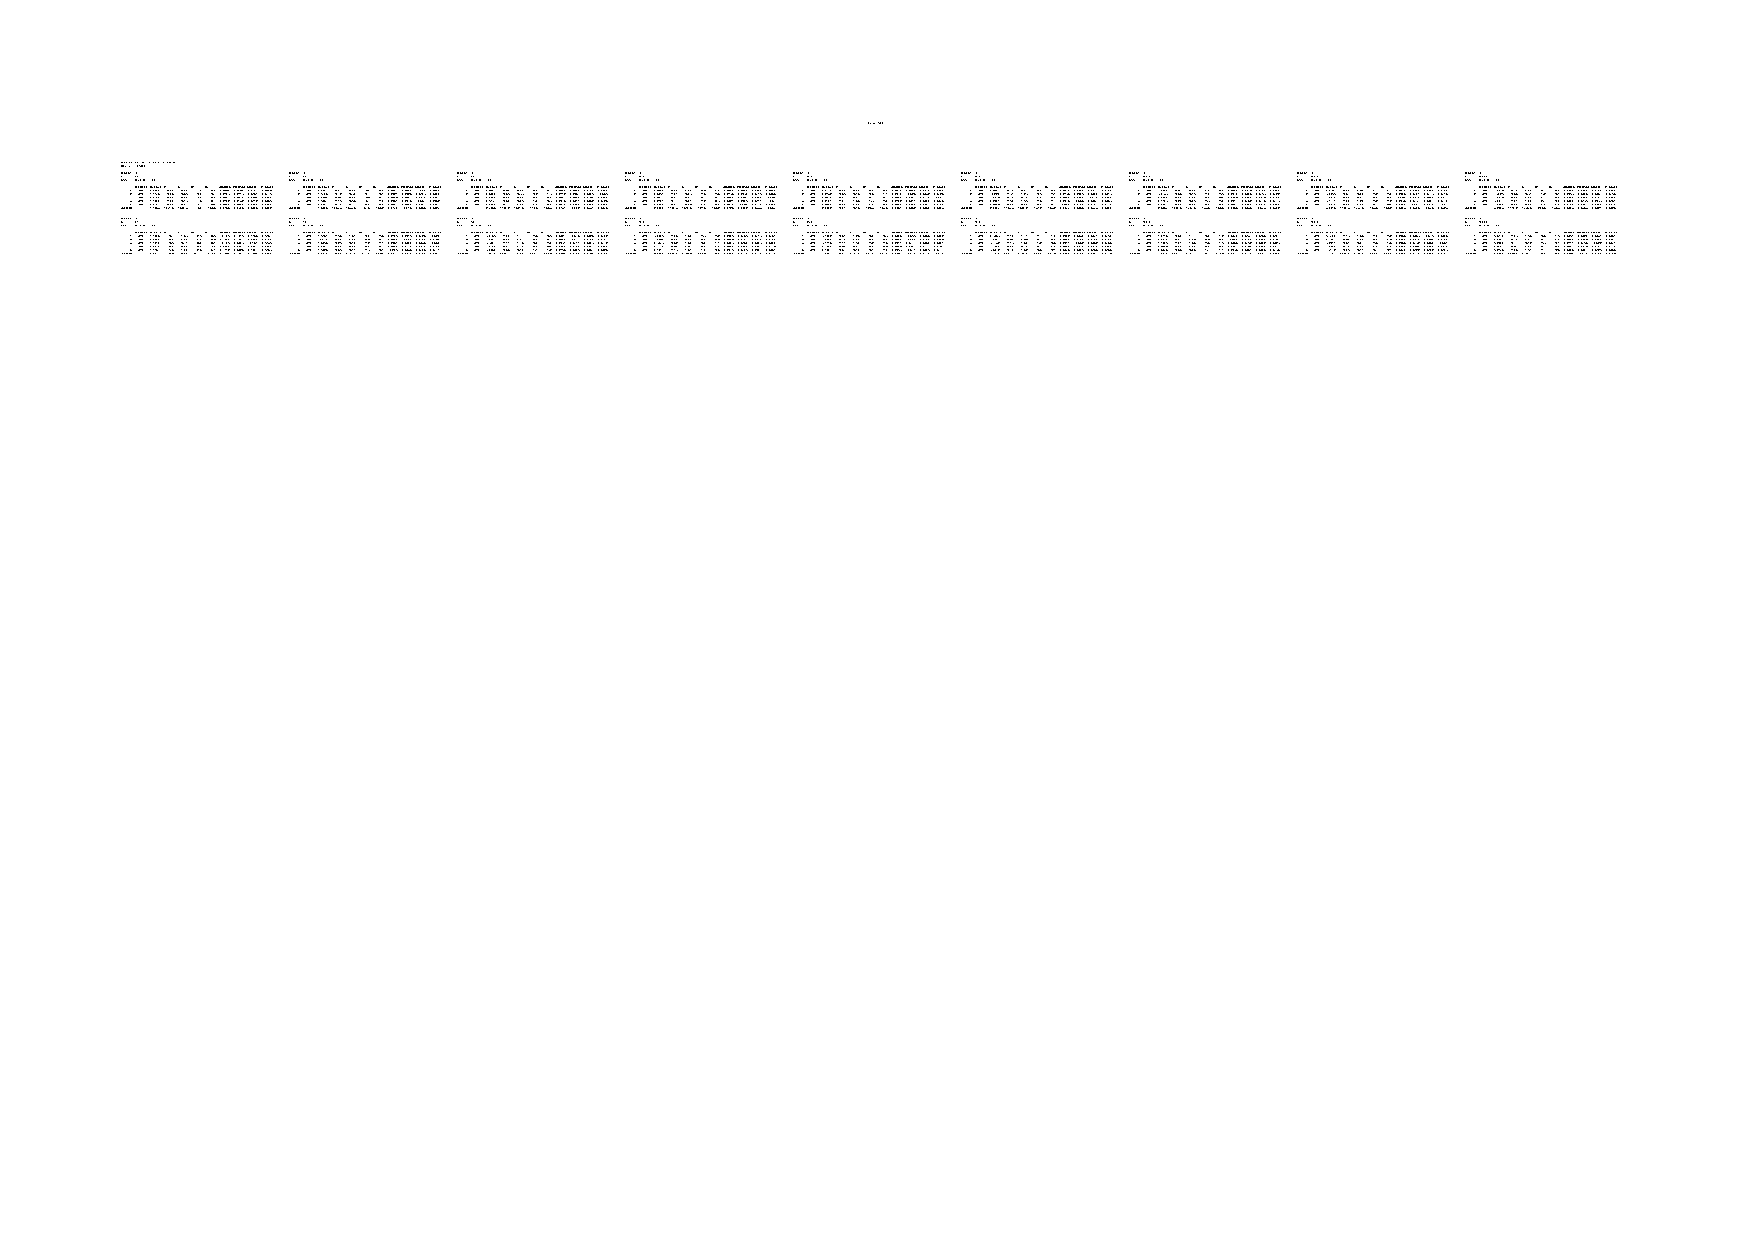
\includepdf[pages={-}, angle=90]{./Second_Phase_Testing/LSVC.pdf}
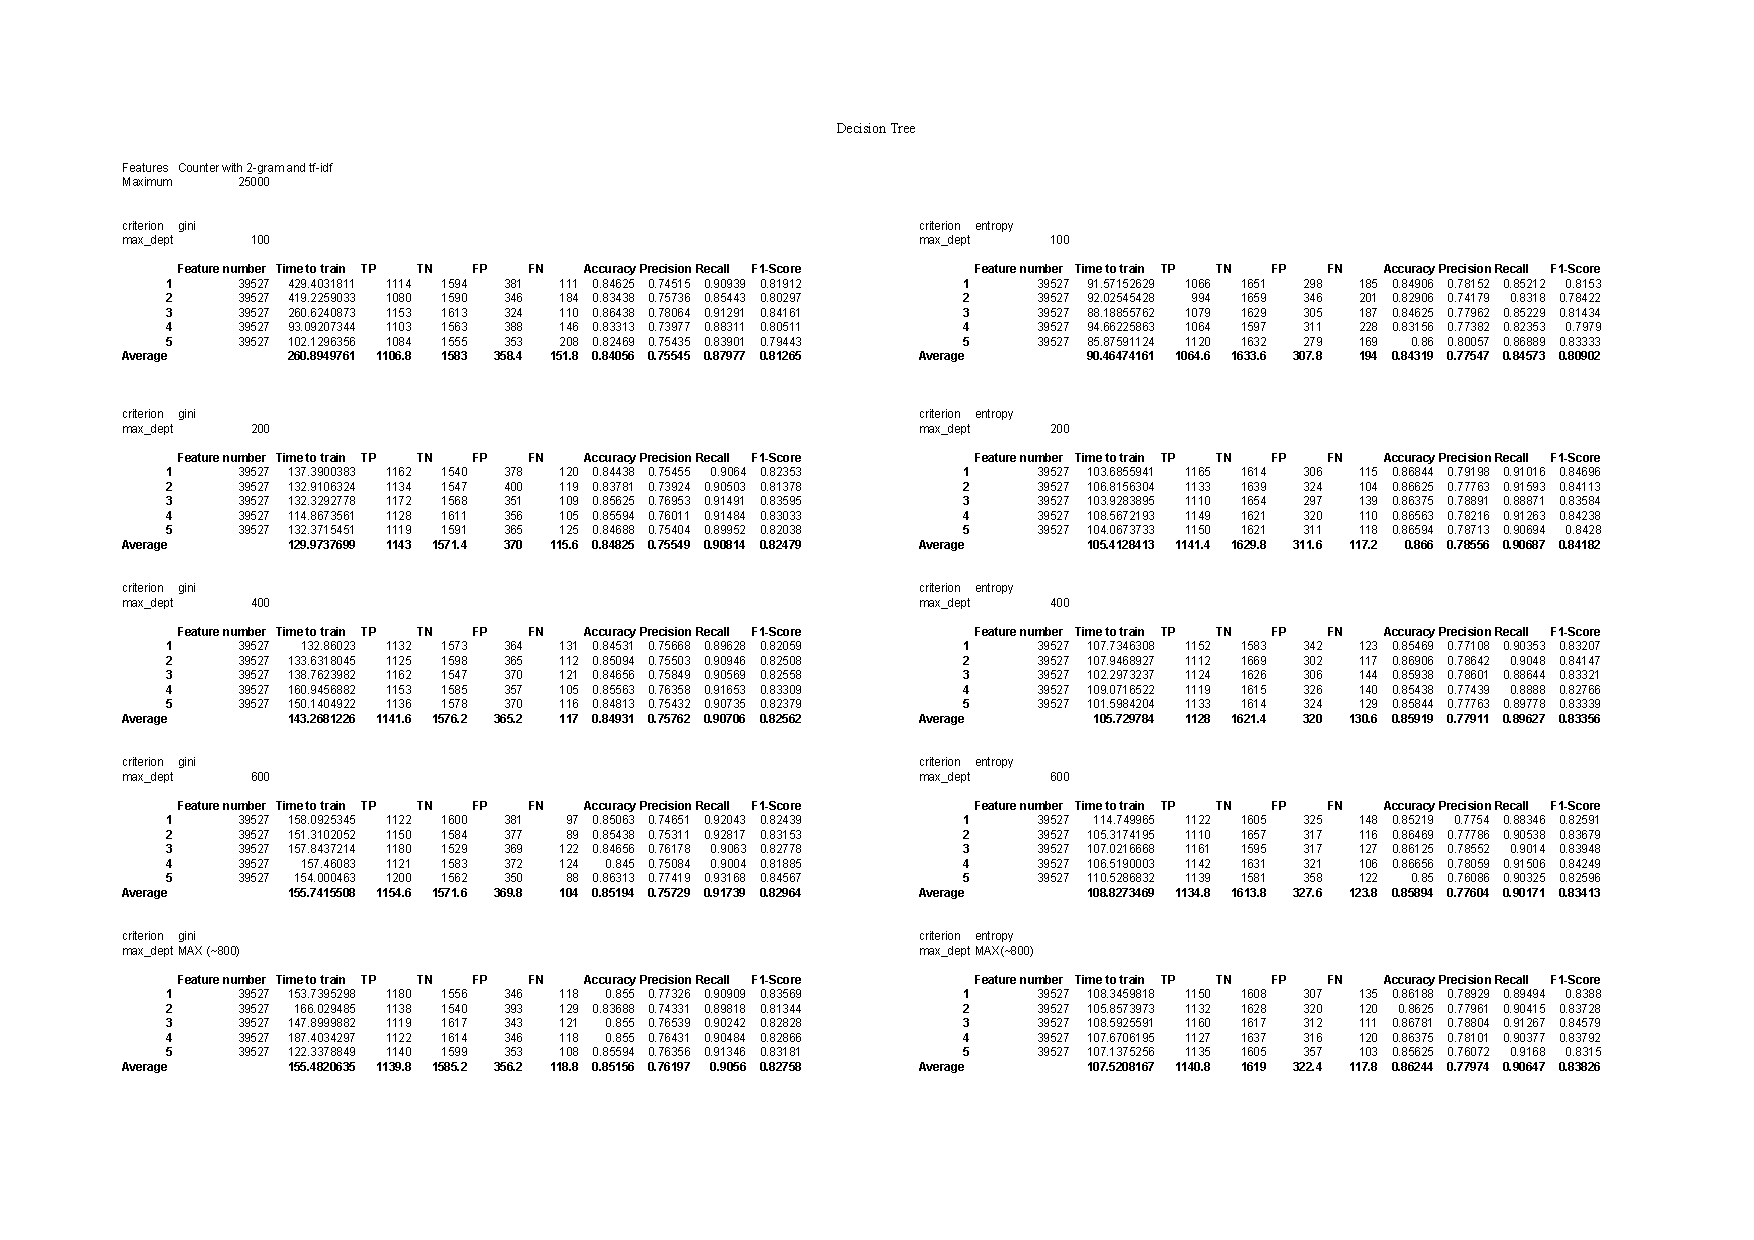
\includepdf[pages={-}, angle=90]{./Second_Phase_Testing/DT.pdf}
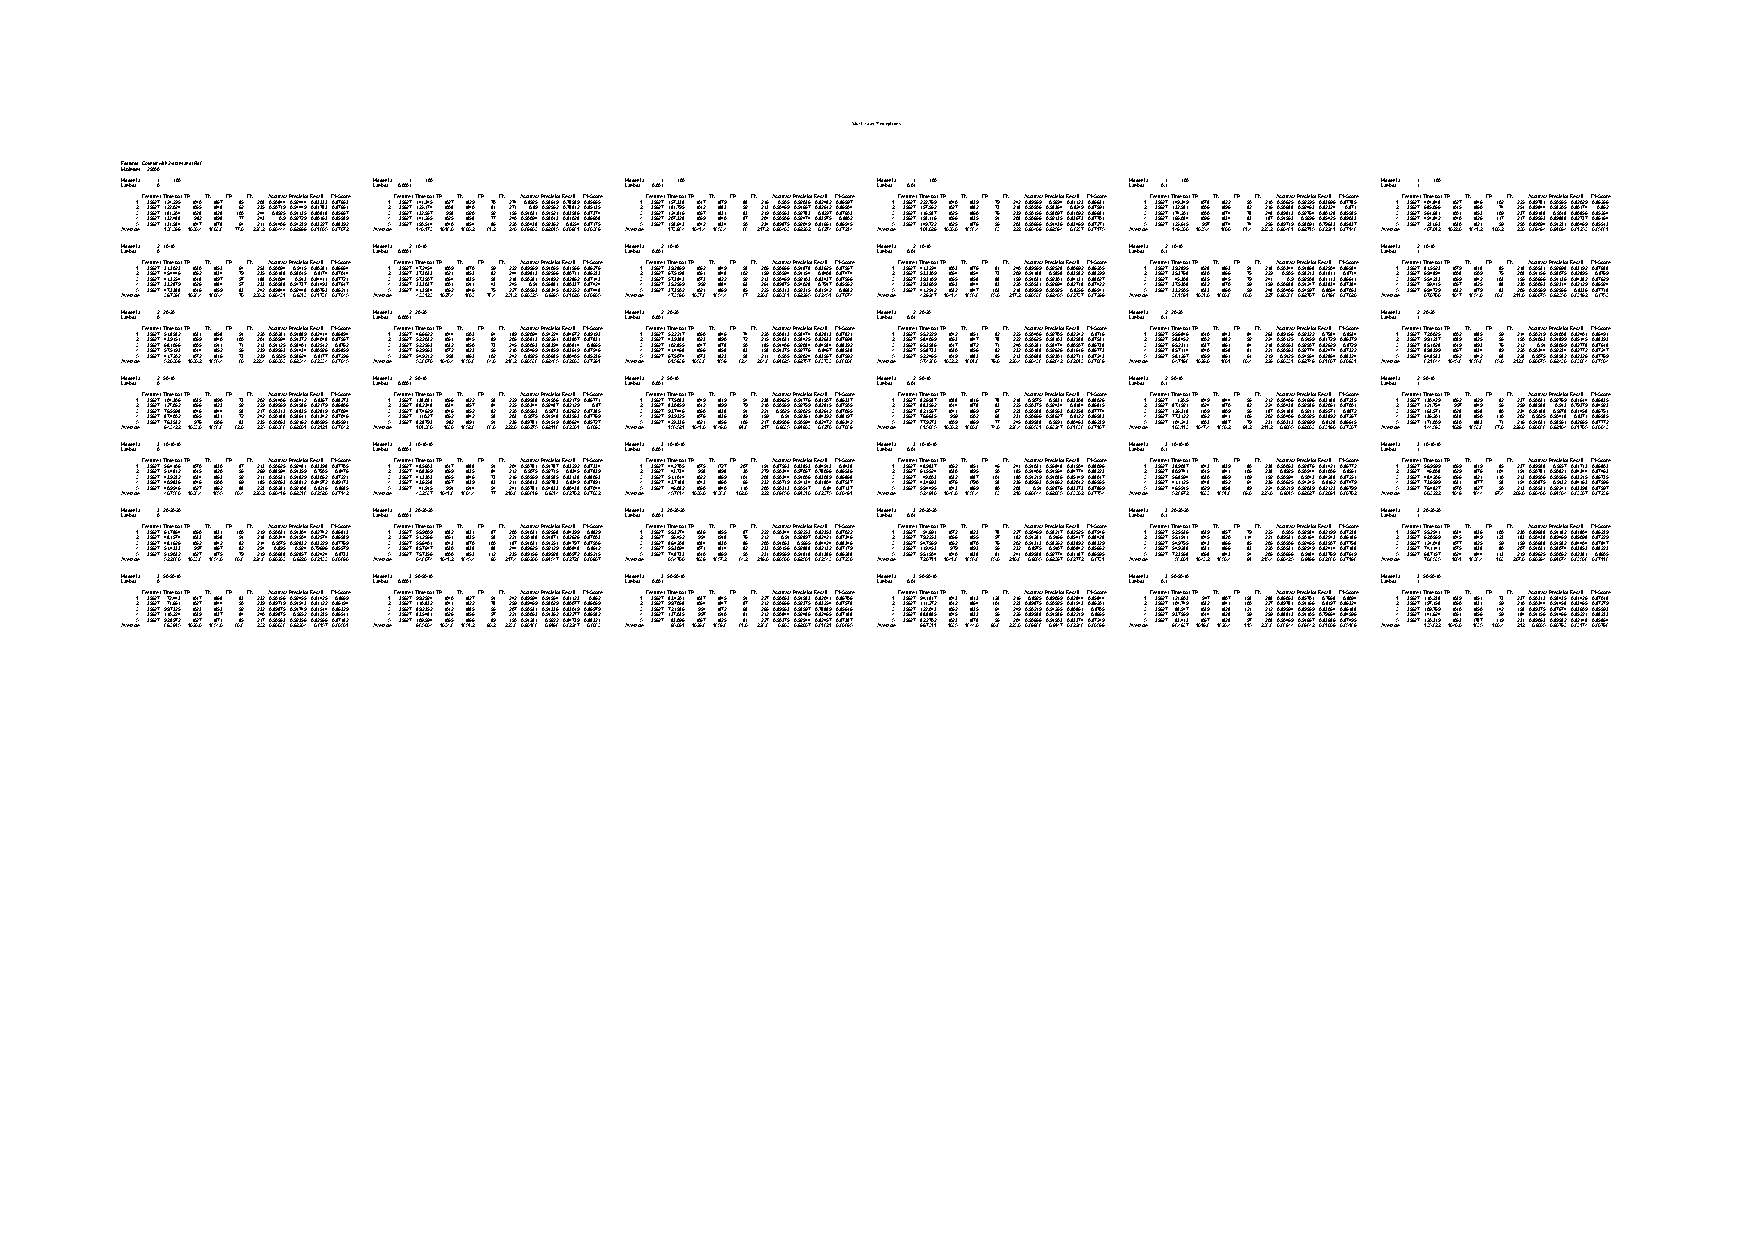
\includepdf[pages={-}, angle=90]{./Second_Phase_Testing/MLP.pdf}


% that's all folks
\end{document}


